\def\year{2020}\relax
%File: formatting-instruction.tex
\documentclass[letterpaper]{article} % DO NOT CHANGE THIS
\usepackage{aaai20}  % DO NOT CHANGE THIS
\usepackage{times}  % DO NOT CHANGE THIS
\usepackage{helvet} % DO NOT CHANGE THIS
\usepackage{courier}  % DO NOT CHANGE THIS
\usepackage[hyphens]{url}  % DO NOT CHANGE THIS
\usepackage{amsthm}
\usepackage{amsmath,amssymb}\usepackage{graphicx} % DO NOT CHANGE THIS
\urlstyle{rm} % DO NOT CHANGE THIS
\def\UrlFont{\rm}  % DO NOT CHANGE THIS
\usepackage{graphicx}  % DO NOT CHANGE THIS
\frenchspacing  % DO NOT CHANGE THIS
\setlength{\pdfpagewidth}{8.5in}  % DO NOT CHANGE THIS
\setlength{\pdfpageheight}{11in}  % DO NOT CHANGE THIS
\newcommand{\citename}[1]{\citeauthor{#1}~\shortcite{#1}}
\DeclareMathOperator{\argmax}{argmax}
\DeclareMathOperator{\argmin}{argmin}

%\nocopyright
%PDF Info Is REQUIRED.
% For /Author, add all authors within the parentheses, separated by commas. No accents or commands.
% For /Title, add Title in Mixed Case. No accents or commands. Retain the parentheses.
 \pdfinfo{
/Title (AAAI Press Formatting Instructions for Authors Using LaTeX -- A Guide)
/Author (Anonymous)
} %Leave this	
% /Title ()
% Put your actual complete title (no codes, scripts, shortcuts, or LaTeX commands) within the parentheses in mixed case
% Leave the space between \Title and the beginning parenthesis alone
% /Author ()
% Put your actual complete list of authors (no codes, scripts, shortcuts, or LaTeX commands) within the parentheses in mixed case. 
% Each author should be only by a comma. If the name contains accents, remove them. If there are any LaTeX commands, 
% remove them. 

% DISALLOWED PACKAGES
% \usepackage{authblk} -- This package is specifically forbidden
% \usepackage{balance} -- This package is specifically forbidden
% \usepackage{caption} -- This package is specifically forbidden
% \usepackage{color (if used in text)
% \usepackage{CJK} -- This package is specifically forbidden
% \usepackage{float} -- This package is specifically forbidden
% \usepackage{flushend} -- This package is specifically forbidden
% \usepackage{fontenc} -- This package is specifically forbidden
% \usepackage{fullpage} -- This package is specifically forbidden
% \usepackage{geometry} -- This package is specifically forbidden
% \usepackage{grffile} -- This package is specifically forbidden
% \usepackage{hyperref} -- This package is specifically forbidden
% \usepackage{navigator} -- This package is specifically forbidden
% (or any other package that embeds links such as navigator or hyperref)
% \indentfirst} -- This package is specifically forbidden
% \layout} -- This package is specifically forbidden
% \multicol} -- This package is specifically forbidden
% \nameref} -- This package is specifically forbidden
% \natbib} -- This package is specifically forbidden -- use the following workaround:
% \usepackage{savetrees} -- This package is specifically forbidden
% \usepackage{setspace} -- This package is specifically forbidden
% \usepackage{stfloats} -- This package is specifically forbidden
% \usepackage{tabu} -- This package is specifically forbidden
% \usepackage{titlesec} -- This package is specifically forbidden
% \usepackage{tocbibind} -- This package is specifically forbidden
% \usepackage{ulem} -- This package is specifically forbidden
% \usepackage{wrapfig} -- This package is specifically forbidden
% DISALLOWED COMMANDS
% \nocopyright -- Your paper will not be published if you use this command
% \addtolength -- This command may not be used
% \balance -- This command may not be used
% \baselinestretch -- Your paper will not be published if you use this command
% \clearpage -- No page breaks of any kind may be used for the final version of your paper
% \columnsep -- This command may not be used
% \newpage -- No page breaks of any kind may be used for the final version of your paper
% \pagebreak -- No page breaks of any kind may be used for the final version of your paperr
% \pagestyle -- This command may not be used
% \tiny -- This is not an acceptable font size.
% \vspace{- -- No negative value may be used in proximity of a caption, figure, table, section, section, section, or reference
% \vskip{- -- No negative value may be used to alter spacing above or below a caption, figure, table, section, section, section, or reference

\setcounter{secnumdepth}{2} %May be changed to 1 or 2 if section numbers are desired.

% The file aaai20.sty is the style file for AAAI Press 
% proceedings, working notes, and technical reports.
%
\setlength\titlebox{2.5in} % If your paper contains an overfull \vbox too high warning at the beginning of the document, use this
% command to correct it. You may not alter the value below 2.5 in
\pdfinfo{
/Title (Interpretable Models of Human Interaction in Immersive Simulation Settings)
/Author (Nicholas Hoernle, Kobi Gal, Barbara Grosz, Leilah Lyons, Ada Ren, Andee Rubin)
/Keywords (interpretable machine learning)
}
%
% Section Numbers
% Uncomment if you want to use section numbers
% and change the 0 to a 1 or 2
% \setcounter{secnumdepth}{0}
% Title and Author Information Must Immediately Follow
% the pdfinfo within the preamble
%
\title{Interpretable Models of Human Interaction in Immersive Simulation Settings}
 \author{Paper ID 134 (this is the rejected AAAI paper)}
 %Nicholas Hoernle,\textsuperscript{\rm 1} 
% Kobi Gal,\textsuperscript{\rm 1}
% Barbara Grosz,\textsuperscript{\rm 2} \\
% \Large \bf Leilah Lyons,\textsuperscript{\rm 3} 
% Ada Ren,\textsuperscript{\rm 4} and Andee Rubin\textsuperscript{\rm 4}\\
% \textsuperscript{\rm 1}University of Edinburgh, 
% \textsuperscript{\rm 2}Harvard Unuiversity, 
% \textsuperscript{\rm 3}New York Hall of Science,
% \textsuperscript{\rm 4}TERC\\
% \{n.s.hoernle, kgal\}@\{sms, inf\}.ed.ac.uk,
% grosz@eecs.harvard.edu,
% llyons@nysci.org, 
% \{ada\_ren, andee\_rubin\}@terc.com}


\newcount\Comments  % 0 suppresses notes to selves in text
\Comments=1

\usepackage{xcolor}
% \definecolor{green}{rgb}{0,1,0}
\newcommand{\kibitz}[2]{\ifnum\Comments=1{\textcolor{#1}{#2}}\fi}
\newcommand{\nh}[1]{\kibitz{blue}{[NH:#1]}}
\newcommand{\kg}[1]{\kibitz{red}{[KG:#1]}}
\newcommand{\bjg}[1]{\kibitz{purple}{[BG:#1]}}

 \begin{document}

\maketitle

% TODO: tense
% TODO: caps all on BFC and FwdSim???

\begin{abstract} 
Immersive simulations are increasingly used for teaching and training in many societally important arenas including healthcare, disaster response and science education.
The interactions of participants in such settings lead to a complex array of emergent  outcomes that present challenges for analysis. 
This paper studies a central element of such an analysis, namely the interpretability of models for inferring structure in time series data. 
This problem is explored in the context of modeling student interactions in an immersive ecological-system simulation. 
Unsupervised machine learning is applied to data on system dynamics with the aim of helping teachers determine the effects of students' actions on these dynamics. 
We address the question of choosing the optimal machine learning model, considering both statistical information criteria and interpretabilty quality. 
Our approach adapts two interpretability tests from the literature that measure the agreement between the model output and human judgment. 
The results of a user study show that the models that are  the best understood by  people are not those that optimize information theoretic criteria.
In addition, a model using a fully Bayesian approach performed well on both statistical measures and on human-subject tests of interpretabilty, making it a good candidate for automated model selection that does not require human-in-the-loop evaluation.
The results from this paper are already being used in the classroom and can inform the design of interpretable models for a broad range of socially relevant domains.
\end{abstract}

% This paper studies the role of interpretability in the design of   models for inferring structure in time series data. 
% We consider unsupervised machine learning that is applied to modeling students interaction in an immersive simulation environment in which  teachers need to understand the effects of the students' actions on the system dynamics. 
% Immersive simulations are commonly used for training in fields such as healthcare and education, but the rich array of emergent outcomes challenges the analysis of participants' interactions.
% We address the question of choosing the optimal model for describing students' activities in an immersive simulation for ecology,  considering both statistical information criteria and interpretabilty. 
% Our approach adapts two interpretability tests from the literature to this setting which measure the agreement between the model output and human judgment. 
% We found that a fully Bayesian approach was shown to provide a good compromise between our human test scores. 
% and the theoretic information criteria, and does not require human evaluation effort. 
% We show that one of the interpretability tests, one where people choose between two competing explanations for a model's output, is preferable to one in which people 
% predict the model output. 
% These results can facilitate the design of  interpretable models for a socially relevant class of domains.
%The results of a user study show that the models that are the most interpretable for people are not those that maximize the information theoretic criteria. 
% the Binary Forced Choice test was a better measure of interpretability than Forward Simulation for our time series setting.
%\bjg{it's not clear to me how identifying the intruder is predicting model outcome; if that's my problem let this stand; otherwise perhaps add something about identifying the outlier in a set of visualizations or similar}\nh{The output is the entire segmentation. So this test focuses on specific instances within the output. Is it clearer if we say: predict a portrayal of the model's output?}  
%Explaining decisions made by AI is an important criteria when designing systems that interact with people. 
%One of the tests (Forward Simulation) requires a human to predict the output of a computational model for a given instance, while the other (Binary Forced Choice) requires a human  to choose one of two possible model outputs for an instance.
% bridges the abstract principles of theory and the firsthand experience of emergent, real-world outcomes.
%and thus even a relatively small set of simulation rules can produce a rich array of emergent outcomes. The range of outcomes expands further when a simulation is participatory and students’ actions influence its course. Being in the simulation is only the first step that needs to addressed. 
%We conduct a user study that compares the goodness of
%fit of different computational models in terms of interpretability and information theoretic criteria. 
%We 
%study the trade-off between choosing the best model according to statistical theory and the model that is more likely to be interpreted by people.  
%\bjg{oops2: is this in comparision to human-in the loop approaches? if so need to say so}. 
% We show that people more readily understand a test where they choose between two competing explanations for a model's output.


\section{Introduction}
\label{sec:introduction}
There is increasing evidence of the value of multi-person embodied simulations for engaging learners in a variety of 
applications, such as healthcare, disaster response and education~\cite{alinier2014immersive,amir2013plan}. 
% Such simulations involve multiple participants simultaneously carrying out actions that change the state of the simulated world. 
Such simulations involve multiple participants simultaneously executing actions that change the state of the simulated world, emulating the social aspect of these problem domains~\cite{smordal2012hybrid}.

For example, consider Connected Worlds\footnote{\url{https://nysci.org/home/exhibits/connected-worlds/}},  the system studied in this paper. Connected Worlds is 
an immersive mixed-reality learning environment 
where students interact with an ecological simulation and learn about the causal effects of their actions over time~\cite{mallavarapu2019connect}. 
% This is the empirical setting used in our paper. \nh{I think this sentence feels really disjoint from the these of the paragraph}
Students' actions have both immediate and long-term effects on the simulation leading to a rich array of emergent outcomes which engender diverse opportunities for learning.
We use Connected Worlds as it provides a good example of an immersive simulation where the simultaneous actions of participants result in complex responses from the system.
%The log file data from Connected Worlds exemplifies how an immersive simulation's state can be tracked as it evolves through time in response to the participants' actions.

Participants in immersive simulations (both instructors and trainees) need to understand how the aggregation of the trainees' individual actions affect the system dynamics over time.
However, no one person can possibly follow what happens, even in a relatively short simulation.  
To provide adequate support for participants, AI systems need to consider not just how well they model the data (e.g., log-likelihood), but also how well people understand the representations that are induced by the models that they employ.

This paper studies the \emph{interpretability problem}: determining the AI model (from a set of candidates) that produces the output that is  best understood by people when it is presented  to them~\cite{gilpin2018explaining,doshi2017roadmap,caruana2015intelligible}. 
We explore a trade-off between the selection of models in an offline manner, to optimize a log-likelihood objective, and the selection of models that maximise an intrepretability score, that is operationalized via experimental tests with people.

The approach consists of the following:
(1) choosing a set of models for describing the effects of participants' activities in the simulation; 
(2) designing tests for computing the interpretability score of a given model applied to Connected Worlds data, based on the agreement between the model output and human judgement; and 
(3) comparing the models selected under statistical measures to the models that are selected to maximise the interpretability score.

%\kg{ NIck, this paragraph is too detailed for the intro. I remove the sentence in 186, too vague, sentence 188 describes step 1 and flows}
%We use time series models to assist with the process of extracting examples, from log file data of an immersive learning simulation, that can be used to encourage the students to discuss and reflect upon their interactions with the simulation.

% \kg{paragraph needs revision. Line 195 makes no sense}
We use hidden Markov models (HMMs) to model the system dynamics, with an additional set of ``sticky'' hyperparemeters which bias the transition dynamics of the latent state space~\cite{fox2008hdp}. 
The input to each model is a multidimensional time series representing the system's responses to students' activities.
The output of the model is a segmentation of the time series into a set of periods, which are contiguous lengths of time during which the system 
dynamics are stable (as judged by the model). Each period thus corresponds to a latent state which persists through time.
% from leilah
%Identifying stable states is useful for our problem domain because they denote periods where the participants were 'holding the course' with a strategy. 
% And if there's room for a second sentence, you might want to bring that back around to how it helps educators, something like:
% If educators know when a given strategy was being adhered to, they can help participants connect strategies to outcomes, and compare and contrast strategies.



%In this domain, we define a period as a length of time where the ecological system displays stable (as judged by the model) characteristics.


% We designed two tests, conceptually described by \citename{doshi2017roadmap}, that determined whether the model was interpretable to people and we applied these tests to our setting. 
%\citename{doshi2017roadmap} defined three classes of test that determine whether a model is interpretable. 
We applied two interpretability tests to our setting, namely the Forward Simulation and Binary Forced Choice tests~\cite{doshi2017roadmap}.
% One test, Forward Simulation, determined whether people could predict correctly the model's output on a specific instance in time;
% the other test, Binary Forced Choice, determined whether people could identify which of two possible model outputs was associated with an unknown data instance. 
% \kg{need to revise following sentence}
The tests visualized a model's output by presenting to people images of the simulation that correspond to periods inferred by the model.

We compared the interpretability score %, as evaluated by a user study, 
of a variety of models by exploring the space of hyperparameter settings.
One of the models, the fully Bayesian model, does not set the value for the hyperparameters but rather treats them as unknown and stochastic variables in the model by placing priors over the hyperparameters.
This model does not require the explicit choice of values of the hyperparameters of interest.

Our scientific hypotheses were that 1) varying the bias hyperparameters of a model would affect its interpretability; and 2) there exists a setting for the bias hyperparameters that would induce an optimally interpretable model. 


The results confirmed Hypothesis 1: there was a variance in model interpretability induced by varying the model hyperparameters. 
In particular, the model that optimized the information criteria did not correspond to the optimally interpretable model according to the interpretability tests. 
% The best results were obtained when using the Binary Forced Choice test.

Hypothesis 2 was partly confirmed, in that there was a region in parameter space that induced higher interpretability scores. We were not able to identify a single parameter setting that was the most interpretable setting. 
The fully Bayesian approach, which does not require any hyperparameter tuning, provided a good balance between interpretability and performance on the theoretical statistical tests.
We argue that this approach can be suitable for situations in which human evaluation testing is infeasible, unethical or impractical.
%available interpretability tests, this approach has merit as it no longer requires the optimisation of a proxy to interpretability that has been noted can produce sub-optimal models~\cite{lage2018human}. 

%S Teachers may wish to discuss students' interactions to highlight salient learning opportunities, but if there are too many ``moving parts'' to the simulation, this becomes a challenging ideal.
%with telecoupled effects that can be removed in both space and time from the point of action. 
% The work forms part of a broader project where the goal is to generate relevant summaries of the CW dynamics such that teachers can effectively engage the students in discussions that stem from their own experiences with the simulation. To achieve this, \textit{we must understand how a model of a system's dynamics maps to human interpretability}. We extend previous work to explore the interpretability of the representations that a Bayesian non-parametric model learns about students' interactions with the CW system.

% Complex systems simulations, such as CW, are becoming increasingly common in formal and informal STEM learning environments~\cite{smordal2012hybrid}. These simulations present scientific phenomena in a manner that bridges principles of science and the firsthand experience of emergent, real-world outcomes. The open-ended and exploratory nature of these simulations presents challenges to teachers' understanding of students' learning. Students' actions  have both immediate and long-term effects on the simulation leading to a rich array of emergent outcomes. Teachers may wish to discuss students' interactions to highlight salient learning opportunities, but if there are too many ``moving parts'' to the simulation, this becomes a challenging ideal. To support these new opportunities for learning, we require the interpretable representations that this paper explores.


% \kg{consider removing the last paragraph}
In studying the interpretability problem applied to a socially relevant class of domains, that of students' interactions in immersive simulation, we make two contributions to the field.
First, we operationalize two interpretability tests and apply them to real-world data. 
%\nh{Do you think this next sentence belongs in the introduction? I am actually happy to have it removed}
%We identify the Binary Forced Choice test as preferable to Forward Simulation in this domain due to its better invariance to the sample noise that might be introduced in the implementation of the tests. 
Second, we show that the fully Bayesian solution shows promise for model selection when access to human experimentation is infeasible. 

The results from this work have already been implemented in a classroom experiment where visualizations of the model's output were shown to the school students who participated with the immersive simulation. The students used the visualizations to bolster their interpretations of events that occurred.


%The visualizations enabled teachers and students to reflect upon and to discuss the strategies that they used while interacting with the simulation; and the students used the visualizations to bolster their interpretations of events that occurred.
%In future work we plan to extend the approach to additional socially relevant real-world settings and to explore how models can be chosen for human interpretability for these settings in an offline manner.


% to operationalize the conceptual Forward Simulation and Binary Forced Choice tests for a popular unsupervised time series model. We further present two results that merit future investigation. First, when seeking an interpretable model, our results suggest that rather than optimising a proxy to interpretability, one should rather use the Bayesian approach of placing a prior on the unknown parameter (thereby effectively integrating it out). Second, we claim that the Binary Forced Choice test is preferable to the Forward Simulation for this implementation.
% Our contributions are twofold. First, we present a mapping from the construct of interpretability to a measurable score. Secondly, we design an experiment that tests the interpretability of a popular time series model. In particular, we model the dynamics of CW with a hidden Markov model wherein latent states correspond to stable states that result from specific actions that the students performed. We investigate the human interpretability of different representations that are learnt by this model and our results suggest that fully Bayesian analysis of model parameters presents a scalable means for selecting a model that (1) accurately captures the distribution of data and (2) provides interpretable representations.

%We examine the trade-off between choosing the best model according to statistical theory and the model that is more likely to be understood by humans. The main result from the human evaluation experiment that we run on Amazon Mechanical Turk is that the fully Bayesian procedure (placing hyper-priors on the hyper-parameters in a model) results in consistently good performance on both statistical measures of predictive performance and on the human interpretability tests, although it is not the optimal choice for either scenario. Our results support the work of \cite{chang2009reading} and suggest that the choice of hyper-parameters, for example the choice of the number of clusters in a clustering algorithm or the choice of topics in a topic model, should not only be optimised for statistical likelihood measures if the goal is to provide interpretable models. However, in cases when human-interpretability-tests~\cite{lage2018human} are not available, using a fully Bayesian analysis presents a good alternative to optimising statistical measures.
%
%In order to optimise an interpretabilty measure, we require that there exists some function that maps the parameter choice to an interpretability score. This function should be (locally) convex for there to exist a region in parameter space that corresponds to a high interpretability score. We test for the existence of this function. Second, we investigate how statistical approximations to this function should be used with caution when attempting to find the true optimal setting for human interpretability. We thus arrive at the following two hypotheses:
%
%\textbf{Hypothesis 1:} \textit{The degree to which a model is interpretable depends on the parameter settings; there exists a region in parameter space that corresponds to a high interpretability score.}
%
%\textbf{Hypothesis 2:} \textit{Optimising parameters for statistical information criteria may not produce the optimal model for human interpretability.}
% \section{Background}



%=========================================================================================
% Methodology ============================================================================
%=========================================================================================
% \section{Methodology}

%We test the human interpretability of a number of models by implementing two tests. The first, Forward Simulation, tests if human subjects can correctly predict the output of a ML model given a visualisation of the input. The second, Binary Forced Choice, tests if human subjects can identify one of two plausible explanations for a ML model's decisions. We build on the experimental design of \cite{chang2009reading} and adapt the design to the time series domain present in CW.

% The period is the unit of state assignment used in this work. We test the interpretability of a period defining \textbf{image intrusion} and \textbf{period intrusion} (analogous to \cite{chang2009reading}'s word and topic intrusion respectively). The notion of image intrusion is an instance of a Forward Simulation experiment and it tests whether an image that does not belong with a collection of other images from one period can be identified by a human. The notion of period intrusion is an instance of the Binary Forced Choice experiment and it tests whether an unknown image can be associated with one of two plausible periods.

% \nh{temporary placeholder for methodology description}
% Our approach consists of the following steps:  
% \begin{enumerate}
%     \item  {Model design}: Choosing set of models $\mathcal{M}$, each  segments a time series of students' activities   into periods.   
%   % \item  {Interpretability measure}: Constructing a  mapping $IS$ that assigns an interpretability score to a given model on a particular dataset.
%   %  \begin{equation*}
%   %      IS: \mathcal{M} \times \mathcal{D} \rightarrow \mathcal{R}
%   %  \end{equation*}
%   % \item Two user study implementations that operationalise the ``Forward Simulation'' and ``Binary Forced Choice'' tests for this domain (Section \ref{sec:method_visualisations}).
%     \item   {Interpretability test}: Designing a test    for computing the  interpretability of a given model $M$ 
%     and dataset $D$ based on human judgment.  
    
    
%      A test returns an interpretability score $IS$  to a given model on a particular dataset. 
%     $IS: \mathcal{M} \times \mathcal{D} \rightarrow \mathcal{R}$
%     \item  {Model selection}: Select the optimal model $M$ on dataset $D$ using a either a statistical information criteria ($IC$) or an interpretability score ($IS$).
%     \begin{equation}
%         \label{eq:model_information_criteria}
%         M^*_C \in \argmin_{M \in \mathcal{M}}(IC(M, D))
%     \end{equation}
%     \begin{equation}
%         \label{eq:model_interpretability_score}
%          M^*_S \in \argmax_{M \in \mathcal{M}}(IS(M, D))
%     \end{equation}
%     % \item   {Model Selection (interpretability)}:  Select  the optimal $M$ on a dataset using 
%     % the interpretability score.   $ M^*_D \in \argmax_{M \in \mathcal{M}}(IS(M, D))$
%     \item  {User Study}: Compare the interpretability of the model chosen from statistical theory to the model that maximises the interpretability score based on the user study.
%     %
% %that maximizes the interpretability score on different data instances.
% %\item  Comparison: Compares the most likely 
%     % the quaA means for selecting periods across different segmentations that are used to test the models' interpretability (Section~\ref{sec:select_segmentation}).
%     % \item A baseline whereby statistical theory is used to select an optimal model  (Section~\ref{sec:baseline}).
%     % \item A comparison of the interpretability of the baseline model to the model that maximises the interpretability score (Section~\ref{sec:interpretability_results}).
% \end{enumerate}
 
% \noindent We proceed to describe each of these steps in turn. 


%=========================================================================================
% Related Work ===========================================================================
%=========================================================================================
\section{Related Work}

This paper relates to a burgeoning body of work on evaluating the interpretablity of machine learning models using human judgment~\cite{rosenfeld2019explainability,gilpin2018explaining,doshi2017roadmap,weller2017challenges}.
%These works vary in how interpretabtility is defined, measured and  evaluated.  
% three tests to quantitatively measure the interpretability of a model's representations.
\citename{doshi2017roadmap} suggested three   tests to evaluate how interpretable a model's representations are to people. 
Forward Simulation: requires the evaluator to predict the output of a model for a given input. 
Binary Forced Choice: requires the evaluator to choose one of two plausible model explanations for a data instance.
Counterfactual Simulation: requires the evaluator to identify what must be changed in an explanation to correct it for a given data instance.
% requires the evaluator to correct an incorrect model output.

In follow-up work~\citename{lage2018human} propose a model selection process that considers both a model's accuracy and its degree of interpretability, given by one of the above tests. 
They provide a framework for iteratively optimizing the interpretability of a model with a human-in-the-loop optimization procedure. Their work applied this framework to a test setting in the lab in which human judgment was used to optimize supervised learning models.
Other works that studied interpretability tests for supervised learning settings include~\citename{wu2018beyond,ribeiro2016should,choi2016retain,lipton2016mythos}.
 
% We extend this work in several ways.
We extend this literature on interpretability in several ways.
First, by adapting the model selection process to an unsupervised learning setting, that of segmenting a multi-dimensional time series into periods. 
Second, by designing specific Forward Simulation and Binary Forced Choice tests that can be applied to data from a real-world immersive simulation. 
%We do not implement the Counterfactual Simulation test due to incompatibility with our domain.
 
Our work was  inspired by \citename{chang2009reading} who were the first to show that optimizing machine learning models in unsupervised settings using predictive log-likelihood may not induce models that are coherent for people.
They focused on the use of topic models for finding meaningful structure in documents and they compared the models that are selected to optimize \textit{perplexity} (analogous to held-out log-likelihood) to the models that were selected by the human interpretability tests that they designed.
% Topics were represented as distributions over words and documents were represented as distribution over topics. 
%A topic model consists of topics, which are distributions over words, and a distribution over these topics for each document.
%The latent structures are commonly referred to as topics to reflect the notion that an informed person can identify the meaningful themes that a document presents. A widely held assumption in this domain is that the predictive log-likelihood of the model (commonly termed \textit{perplexity} in the topic modeling literature) on held-out data presents a valid metric for evaluating the quality of the model~\cite{blei2003latent,teh2005sharing,hoffman2010online,chang2009reading}. In \citename{lage2018human}'s terminology, the perplexity is the interpretability proxy in these works.
%When interpretability is the goal, then 
% It is important to emphasise that topic models are unsupervised models. They find plausible structure in the text documents and, when interpretability is the goal, 
%the topics should align with a reader's notion of a topic. There is therefore no ground truth to the representations that these models learn. The models that we discuss in this investigation are similarly unsupervised with no ground truth.

 
\citename{chang2009reading} operationalized two Forward Simulation tests for evaluating the interpretability of a topic model: word intrusion, in which the evaluator is required to identify which of several words does not belong together in one topic represented by the other words; and  topic intrusion, in which the evaluator is required to 
identify which of several topics is not associated with a given document.
%They found that topic models which optimize statistical measures (log-likelihood, perplexity?) are not the most coherent models to people. 
We extend this work 
% by adopting an interpretability framework 
to a multi-dimenstional time series domain and we introduce a Binary Forced Choice test to complement the ``intrusion'' Forward Simulation test.

%- given one coherent topic, a human test subject is required to identify which word does not belong with that topic. {Topic intrusion} - given a document with a number of high probability topics that describe that document, the test subject must identify which topic does not describe the document.
 
% incorporating human judgement into the model learning 
% frameowrk
% \noindent Word intrusion was tested by presenting human evaluators 6 words where 5 words have a high probability under a given topic and 1 word, the \textit{intrusion}, has a low probability under that topic. The evaluator chooses which word he/she believes does not belong in the group. For the topic intrusion test, a document is presented as a distribution over topics. For each document, three high probability topics are presented next to one low probability topic, where each topic is represented by the 4 most probable words under that topic. The evaluator is required to select the topic that is not associated with the document.


% We follow \citename{rosenfeld2019explainability} and refer to the term ``interpretability'' in this paper as a function that takes as input a model and a data record and returns a representation of the model's logic. We propose that the ``explicitness'' of this interpretability function, the degree to which the model's interpretability is understandable to the intended user, can be measured by the implementation of interpretability tests~\cite{ribeiro2016should}. The tests that we propose add to the literature on interpretability that optimizing proxies for interpretability can lead to the selection of models that are sub-optimal, in terms of how interpretable an unsupervised model's representations are to human end-users.

% \subsection{Optimizing Proxies for Interpretability}

% It is common in the literature to learn a model that aims to be interpretable by optimizing a proxy that can be directly computed from the model~\cite{lage2018human}. For example, a proxy might be the number of parameters in a model and one might optimize a L1 penalized loss function to optimize over the model fit to the data while enforcing a constraint of fewer model parameters. In a different example, a proxy supposes that a class of models are more interpretable than another; \citename{wu2018beyond} used decision trees to reqularize the decision boundaries of neural networks. 

% \citename{chang2009reading} was the first study to explicitly conclude that optimizing a proxy, held-out log-likelihood in this case, did not correspond to optimizing the model's interpretability. More generally, \citename{lage2018human} conclude that optimizing the incorrect proxy can lead to worse interpretability results than finding a sub-optimal model but using the correct proxy. 


% % \subsection{General Interpretability Tests}


% \noindent \citename{hilgard2019learning} take a novel perspective on interpretability and suggest that ML systems can simply convey signals about a complex environment via representations that humans are familiar with.




%=========================================================================================
% Connected Worlds =======================================================================
%=========================================================================================

\begin{figure}[t]
\centering
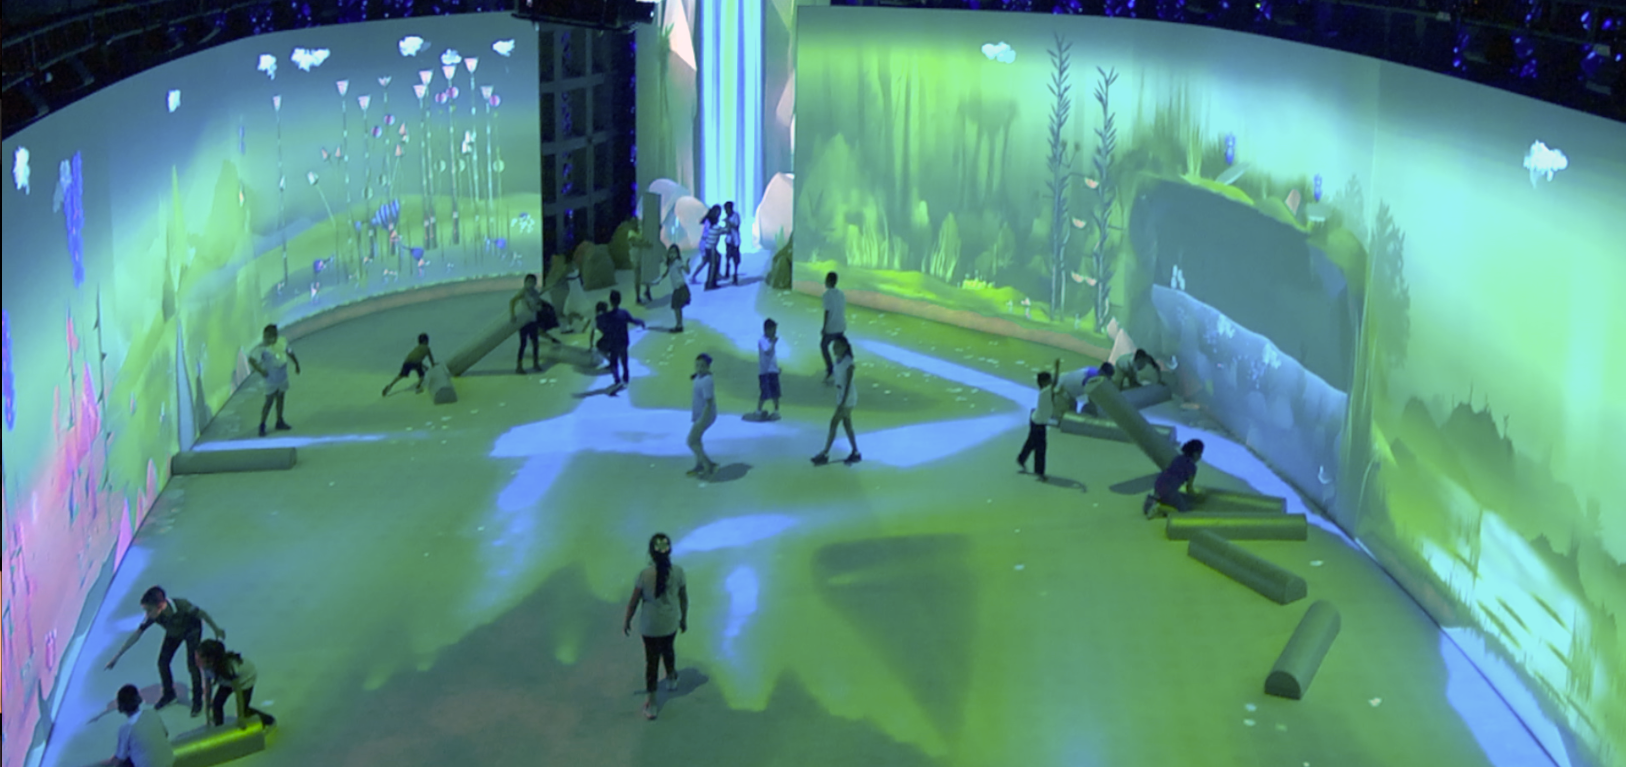
\includegraphics[width=0.48\textwidth]{./images/cw_viz2.png}
\caption{Picture of the floor of Connected Worlds; facing the Waterfall from the area labelled ``Floor'' in Figure~\ref{fig:connected_worlds_graphic}.}
\label{fig:connected_worlds_viz}
\end{figure}


\section{The Connected Worlds Domain}
\label{sec:cw_desc}
Connected Worlds (CW) is a multi-person ecology simulation (installed at a science museum that hosts classes on field trips,) and has the goal of teaching students about complex systems and systems thinking. 
It is an immersive environment-simulation comprising four biomes (Desert, Grasslands, Jungle \& Wetlands) that are connected by a central flow of water, fed by a waterfall. The simulation exhibits large scale feedback loops and presents the opportunity for participants to experience how their actions can have (often unintended) effects that are significantly removed in time and/or space. Students plant trees which flourish or die, animals arrive or depart, and rain clouds form, move through the sky and deposit rain into the waterfall. 
Figure~\ref{fig:connected_worlds_viz} shows a photograph of the CW space where participants are seen to be interacting with both physical and virtual objects in the simulation.

Students interact with CW by physically moving plush logs to control the direction of water that flows in the simulation. Water can be directed to each of the four biomes and the distribution of flowing water depends on the placement of the logs. Water enters the simulation via rainfall events which are out of the students' control. These release water into the waterfall (to replenish the primary source of water) and into the individual biomes.

\begin{figure}[t]
\centering
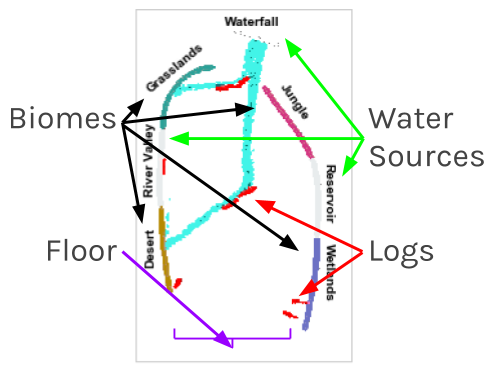
\includegraphics[width=0.48\textwidth]{./images/cw_snapshot.png}
\caption{CW snapshot view. Biomes are labelled on the perimeter and logs appear as thick red lines. Water (blue stream in the middle of the image) enters via the waterfall and in this image it mainly flows toward the Grasslands and the Desert.}
\label{fig:connected_worlds_graphic}
\end{figure}

The nature of the simulation is complex on a variety of dimensions as it involves a large number of students simultaneously executing actions that change the state of the simulated environment. Thus, each participant will have a different view of what transpired, depending on the actions s/he took and the state changes that resulted. 
It is therefore important to develop tools that can support  the understanding of the students' interactions in complex environments such as CW. 
Such tools can  support teachers and students in reflecting upon and generalizing from their simulation experience.
% \kg{we don't show the below}\nh{also trying to stay away from the use of "system dynamics" - I think it is mostly "flow" now}
% A model that highlights stable periods of system dynamics could help teachers and the  class reflect upon the students' teamwork in dividing water equitably, and on the impact of water inequity on the larger ecosystem. 

% \subsection{Data from CW}
A data set ($D$) consists of 8-minute long sessions where students interact with CW. 
For each session, the system logs the water levels in the simulation at a 1Hz frequency, forming a time series that describes the effects of the students' actions on the water flow in the simulation.  
%Each line of the log corresponds to a second of interaction in CW and a session is 8 minutes long. 
CW also provides 
%One interaction session with CW corresponds to an 8 minute period where one class of students interacted continuously with the simulation.  The simulation also provides 
a visual representation of the system state, referred to as the \emph{session view}; a snapshot from this representation is shown in Figure~\ref{fig:connected_worlds_graphic}.
% Figure~\ref{fig:connected_worlds_graphic} shows a session view of CW at a given point in time. 
We use two controlled sessions of students interactions with CW.\footnote{Access to the data files is currently restricted but can be granted upon request.}\footnote{We followed an approved IRB protocol for the collection of our data.}


% This visual representation is a \textit{.MOV} file where each second in the file contains an image that corresponds to the same time in the \textit{.CSV} file. In this way, there is a mapping from time in the \textit{.CSV} to an image representation at that point in time from the \textit{.MOV} file. An example of an image representation in the \textit{.MOV} file is shown in Figure~\ref{fig:connected_worlds_graphic}.

% \begin{figure}[t]
% \centering
% 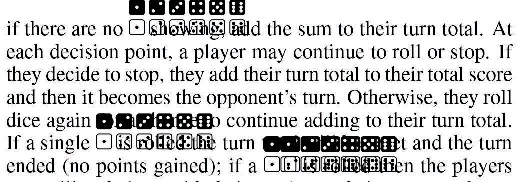
\includegraphics[width=0.9\columnwidth]{figure1} % Reduce the figure size so that it is slightly narrower than the column. Don't use precise values for figure width.This setup will avoid overfull boxes. 
% \caption{Using the trim and clip commands produces fragile layers that can result in disasters (like this one from an actual paper) when the color space is corrected or the PDF combined with others for the final proceedings. Crop your figures properly in a graphics program -- not in LaTeX}
% \label{fig1}
% \end{figure}

% \begin{figure*}[t]
% \centering
% 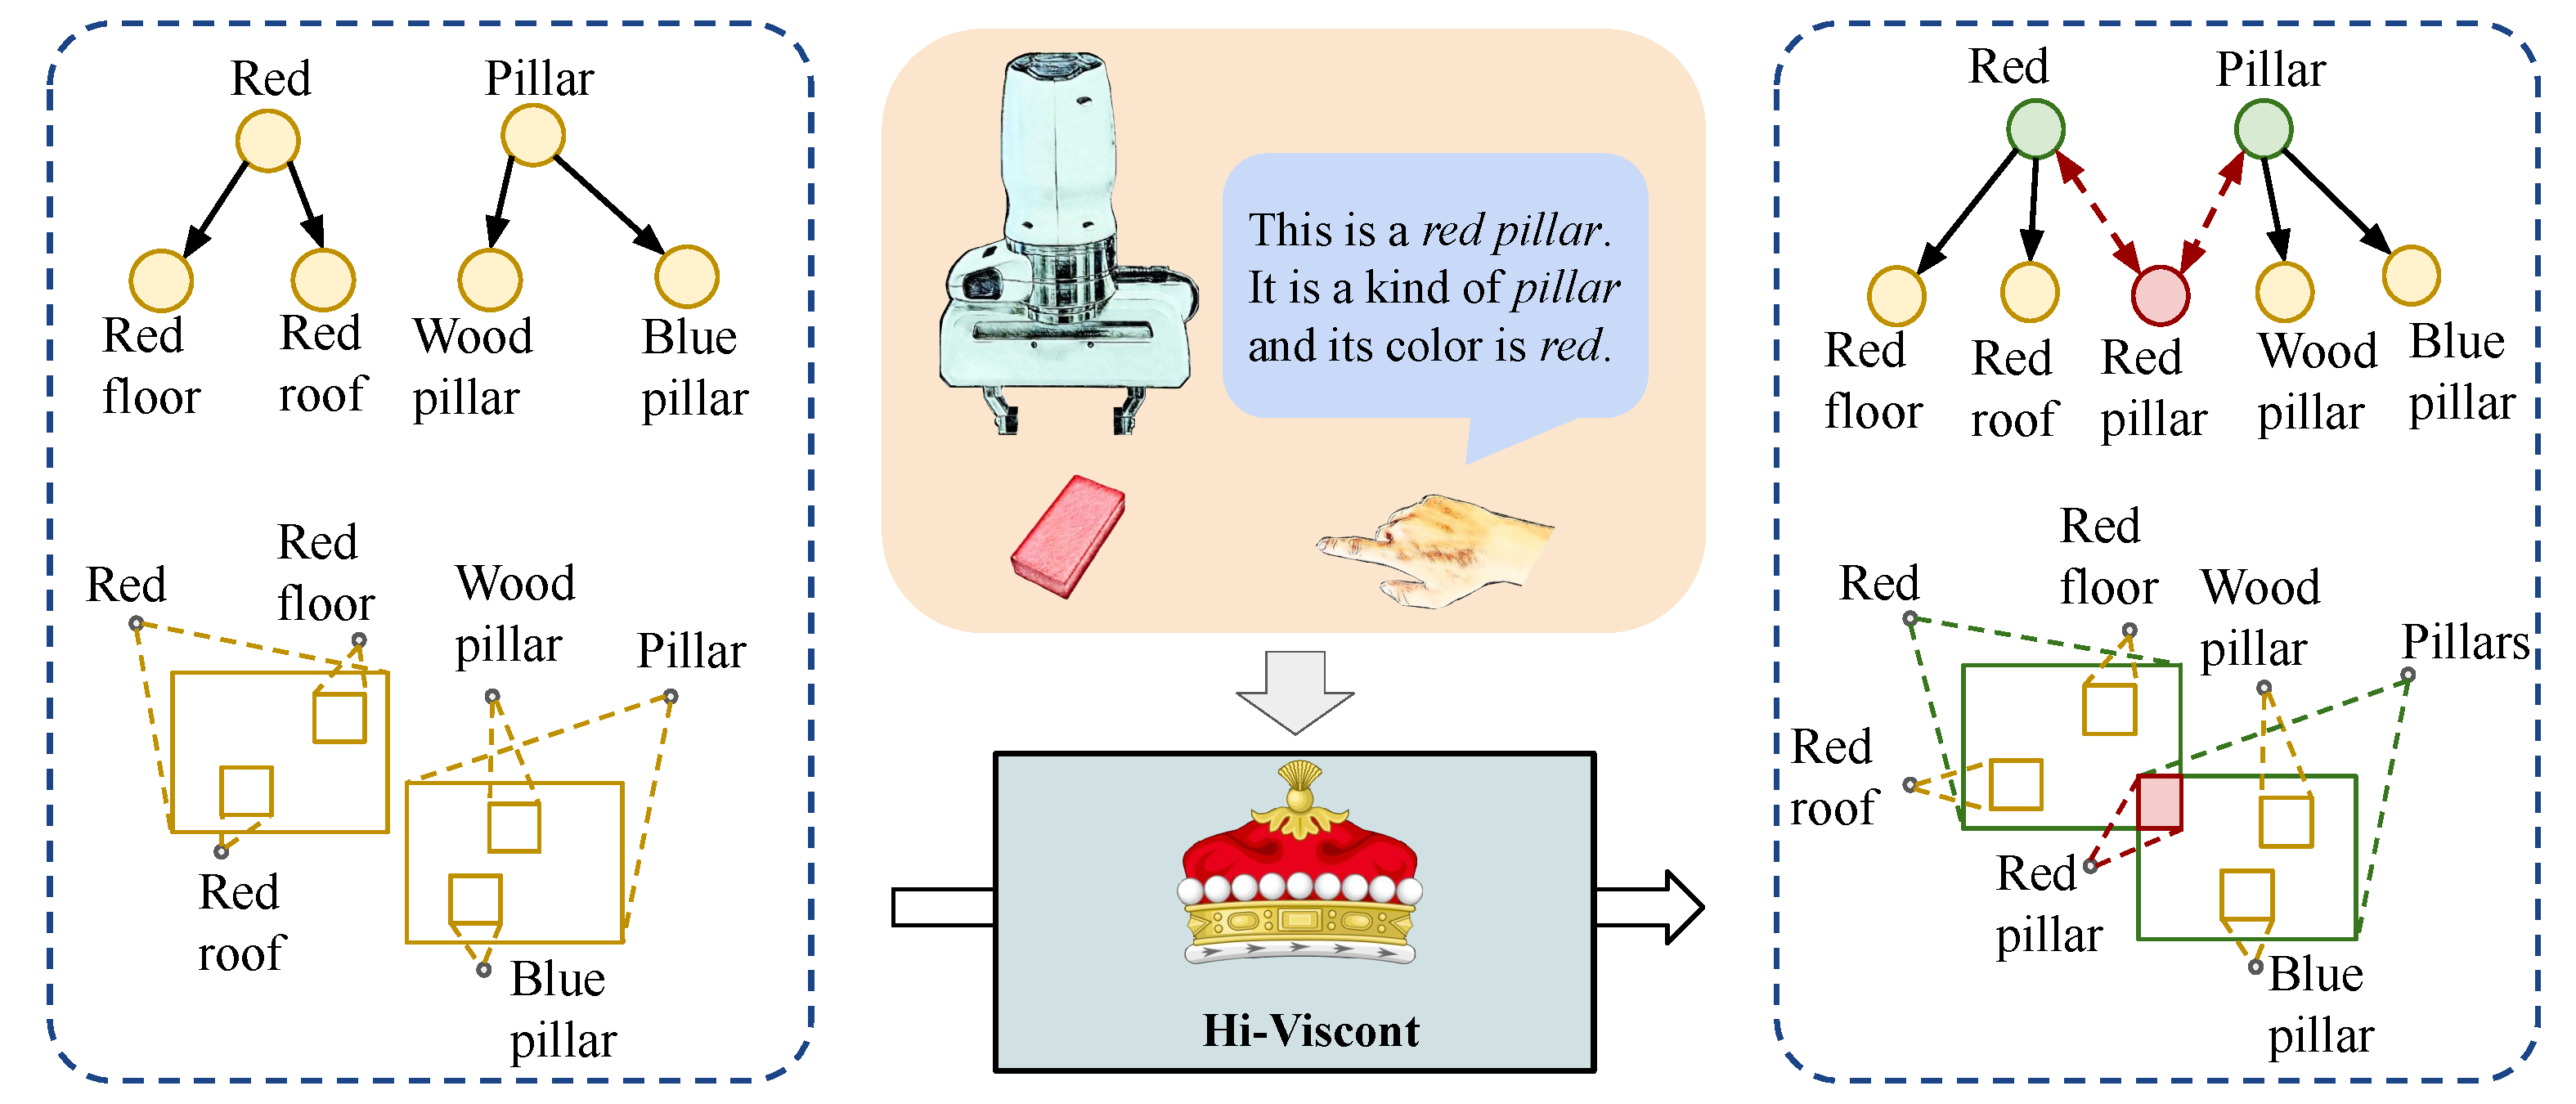
\includegraphics[width=0.8\textwidth]{figure2} % Reduce the figure size so that it is slightly narrower than the column.
% \caption{Adjusting the bounding box instead of actually removing the unwanted data resulted multiple layers in this paper. It also needlessly increased the PDF size. In this case, the size of the unwanted layer doubled the paper's size, and produced the following surprising results in final production. Crop your figures properly in a graphics program. Don't just alter the bounding box.}
% \label{fig2}
% \end{figure*}



\section{Measuring Interpretability}
\label{sec:interpretability_tests}

\begin{figure}
\centering
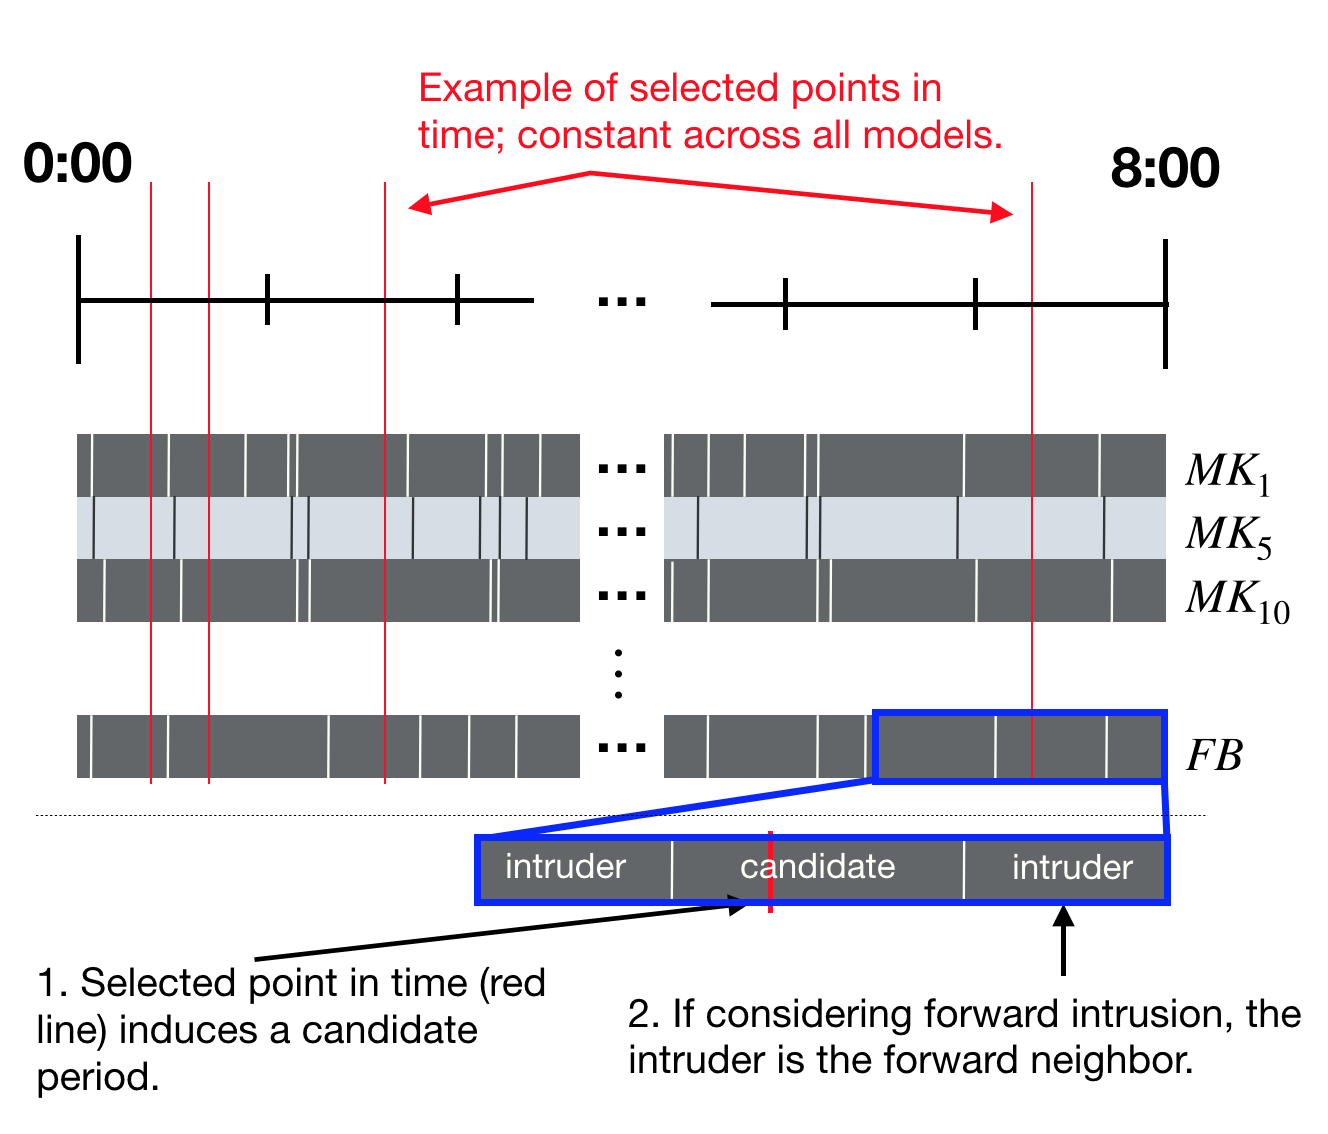
\includegraphics[width=0.45\textwidth]{images/period_selection_representation}
\caption{
\textbf{Top:} segmenting a time series into periods. The data series is represented as a horizontal line from minute 0 to 8; red vertical lines denote sampled time points in the time series; each model is shown as a grey rectangle; models segment time series into periods delimited by white vertical lines. \textbf{Bottom:} the forward or backward neighbour of the candidate period is selected as an intruder.}
\label{fig:selection_representation}
\end{figure}

\begin{figure*}[t]
\centering
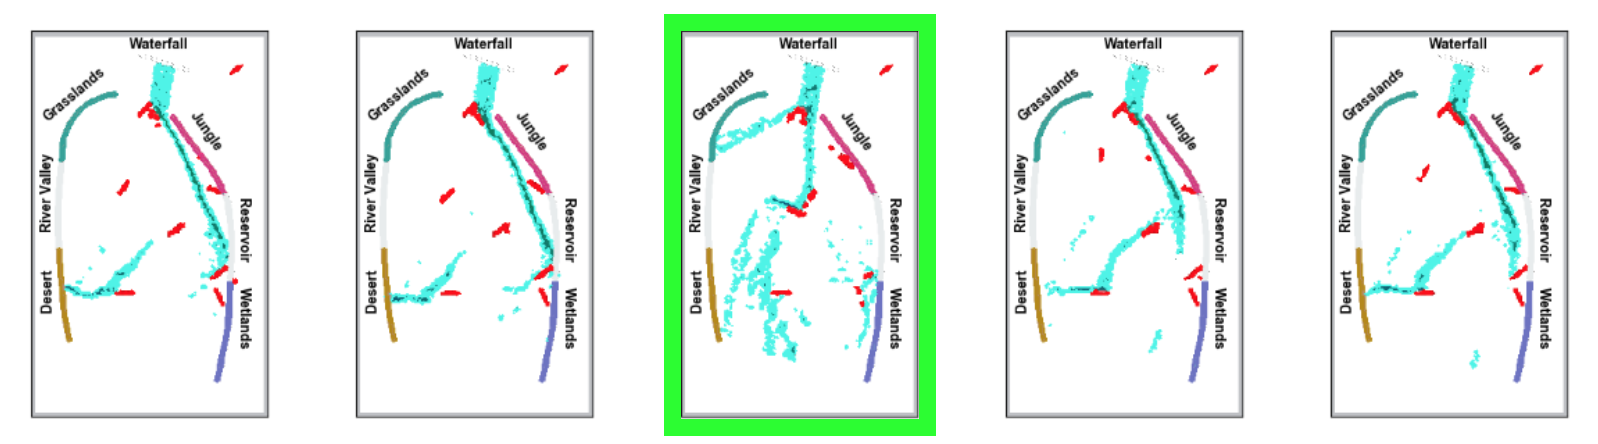
\includegraphics[width=0.75\textwidth]{images/test1_screenshot}
\caption{Screenshot of the  Forward Simulation  test interface. Here $4$ of the images show water flowing towards the Wetlands with a small stream being directed to the Desert. An intruder image, the highlighted one, shows water flowing to the Grasslands and there is neither water flowing to the Wetlands nor to the Desert in this image.}
\label{fig:test1_screenshot}
\end{figure*}

We use an interpretability score $IS$ to measure the interpretability of a model $M$ applied to a data set $D$ ($IS: M \times D \rightarrow \mathcal{R}$).  
The interpretability score is operationalized via an interpretability test which takes as input a model segmentation of a time series (into periods) and a selected point in time $i$ from the time series.
Each test consists of a \emph{visualization} which presents any period as a set of images extracted from the session view.
A test instance returns True if an evaluator successfully completes the required objective. For the   Forward Simulation test, the objective is to correctly simulate the model output for a given instance. For the Binary Forced Choice test, the objective is to correctly  identify the best model output that matches a given instance.
%in Binary Forced Choice test.
%\kg{need to revise the below, candidate and intrusion have not been defined}

% is able to distinguish between the intrusion period and the candidate period using the visualization.
% \bjg{is above true of all interpretability tests or only the forward prediction? In any case, need to move Fig 4 and Fig 5 up here as examples somehow or at least some abstract description of them...} 

% \item ``Counterfactural simulation'' present possible explanations and test whether or not the human can correct the explanation for the instance of data.
% \end{enumerate}
% \noindent We operationalize the Forward Simulation and the Binary Forced Choice tests for the domain of CW. Since the CW domain contains a mapping from time to image representation, we leverage the visual representation of the state of the simulation (e.g., Figure~\ref{fig:connected_worlds_graphic}) to present to the human test subjects: Any time $i$ has a corresponding image representation.

%which each implement the definition of the respective tests. A selected point in time, $i$, is used to choose a candidate period; where the candidate period is the period that is active at time $i$.
%We say that a  period is \textbf{active} for model $M$ at time $i$ if model $M$ uses  the period   to describe the dynamics of the data at that point $i$. 

We adapted the Forward Simulation and Binary Forced Choice tests~\cite{doshi2017roadmap} to the CW domain using the notion of \textit{candidate} and \textit{intrusion} periods.  
%Given a  time point $i$ is used to select a \emph{candidate period} from the model's segmentation and an \emph{intrusion period} that is different than the candidate period.
%If at time $i$, model $M$ uses period $p$ to describe the dynamics of the data, 
We say that period $p$ is \textbf{active} for model $M$ at time $i$ if  $M$ infers the period $p$ to describe a contiguous length of time in the time series, and $p$ includes the time $i$.
Figure~\ref{fig:selection_representation} shows how a time point (red vertical line) is used to select a candidate period where the candidate period is the active period from model $M$ at $i$ (the active period for a model intersects with the red line).

Hypothetically, the intruder can be any period in a model's segmentation of the time series. 
However, intrusion periods that are further away in time from the candidate period would be easier to detect due to the non-stationary evolution of the system. 
We make a design decision to chose the period that is immediately adjacent to the candidate period, either forward or backward in time, thereby testing the specific choice of boundary between the two periods. 
Figure~\ref{fig:selection_representation} (bottom) shows that the intrusion period is selected as the neighbor to a candidate. 


Figure~\ref{fig:test1_screenshot} shows an example of the Forward Simulation test.
This test sampled 4 session-view images from the candidate period of $M$ at $i$, and a single session-view image for the intrusion period. 
The images were presented in a random order.
The test evaluator was required to identify which image was the intrusion image. 
% \nh{Kobi, above, I have overloaded the use of simulate. The one use is "The CW simulation" the other use is the "Forward Simulation". We need it when referring to "Forward Simulation" (as that is Doshi-Valez's terminology) but is this use above clear that I am referring to this same "Forward Simulation". The whole point of the above comment is to address the query that the selection of an intruder image corresponds to one simulating an instance of the model output.}
In Figure~\ref{fig:test1_screenshot}, the image that is outlined in green is the intrusion image that corresponds to the intrusion period.
Since the output of model $M$ is a segmentation of a time series into periods, if the test evaluator could distinguish between the candidate and intrusion periods, this corresponds to them simulating the choice of two of these periods.


Figure~\ref{fig:test2_screenshot} presents an example of the Binary Forced Choice test. 
The test displays an unknown session-view image from a candidate period (center of screen) and two competing explanations for this image (``Period 1'' or ``Period 2''). 
Each of the  two competing explanations is visualized as four images sampled from the candidate or the intruder period.
The unknown image is sampled in time close to the boundary of when the candidate period transitions into the intruder period (or when the intruder period transitions into the candidate period if the order was reversed).
A test evaluator is required to choose between the two competing explanations.
In Figure~\ref{fig:test2_screenshot}, Period 1, highlighted in green, is the correct choice of explanation for the unknown image.


Given data set $D$ and model $M$, the interpretability score $IS$ of a model is equal to the expectation   of the test over sampled points in a time series $D$.
\begin{equation}
    \label{eq:interpretability_score_eq}
     IS(M,D) = E_{i\sim D} [ T (M,D,i)]  
\end{equation}
Where $T(M,D,i)$  denotes the average test score (over all evaluators) of model $M$ on data set $D$ at sampled point in time $i$. The set of time points $\{i\}$ were uniformly sampled from the time series with the additional constraint that each minute of interaction had at least one sample.
%As is depicted in Figure~\ref{fig:selection_representation}, 
For every model we test, we hold constant the selected times $\{i\}$ in the time series. In this way we  control for different areas in the time series being more or less difficult to segment.

%\kg{move to user study?}
%Each test trial presents to a test subject a single \textit{(candidate period; intrusion period)} pair, selected at time $i$. Since the interpretability score $IS$ is a measure on the entire data set $D$, we require multiple samples of $i$ through time for each data instance and $IS$ is the average of the scores of these samples. 
%Further, 
% Figure~\ref{fig:selection_representation} again shows how $i$, the vertical red lines, are held constant across model conditions.
% \kg{the following wasn't clear}Here, one image is selected from the candidate period but it is chosen to be $1$ time step away from the period boundary (where the intrusion period begins). This image, the unknown image, is presented in the center of the visualisation.

% Here, we present $5$ images to a human test subject where $4$ images are selected from the candidate period and $1$ image, the \textit{intrusion image}, is selected from the intrusion period. The test subject is required to identify which image is the intrusion image, thereby simulating the model output. The average ability of test subjects to correctly identify the intrusion image is the $T(M,D,i)$ score where $T$ is the Forward Simulation test and $i$ is the instance in time used to select the the candidate and intrusion periods. In Figure~\ref{fig:test1_screenshot}, the image that is outlined in green is the intrusion period.


\begin{figure*}[t]
\centering
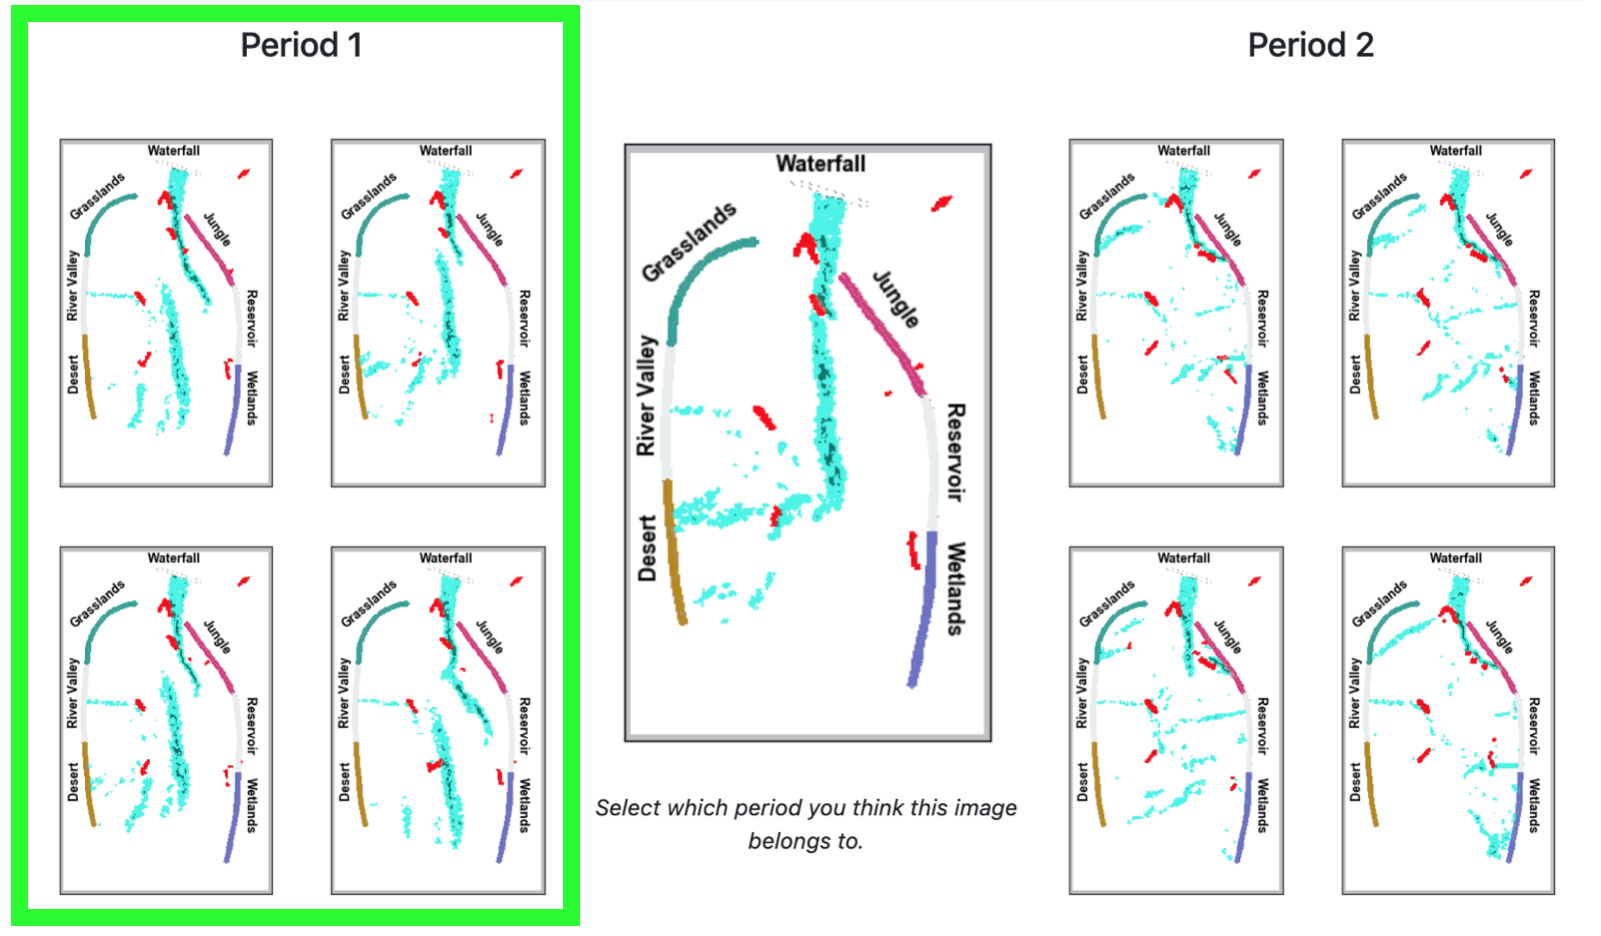
\includegraphics[width=0.70\textwidth]{images/test2_screenshot}
\caption{Screenshot of the  Binary Forced Choice  user interface. An unknown center image needs to be associated with either ``Period 1'' or ``Period 2''. In this case, streams of water flowing to both the Grasslands and to the Jungle capture the dynamics in Period 2. Period 1 has a small amount of water reaching the Desert which is consistent with the unknown image.}
\label{fig:test2_screenshot}
\end{figure*}

% The period is the unit of state assignment used in this work. We test the interpretability of a period defining \textbf{image intrusion} and \textbf{period intrusion} (analogous to \cite{chang2009reading}'s word and topic intrusion respectively). The notion of image intrusion is an instance of a Forward Simulation experiment and it tests whether an image that does not belong with a collection of other images from one period can be identified by a human. The notion of period intrusion is an instance of the Binary Forced Choice experiment and it tests whether an unknown image can be associated with one of two plausible periods.

% \noindent We require the following components for the implementation of this study:
% \begin{enumerate}
%     \item A set of models $\mathcal{M}$ that segment the data into periods (Section~\ref{sec:segmenting_time}).
%     \item A measure of the interpretability of a model (Section~\ref{sec:interp_score}).
%     \item Two user study implementations that operationalise the ``Forward Simulation'' and ``Binary Forced Choice'' tests for this domain (Section \ref{sec:method_visualisations}).
%     \item A means for selecting periods across different segmentations that are used to test the models' interpretability (Section~\ref{sec:select_segmentation}).
%     \item A baseline whereby statistical theory is used to select an optimal model  (Section~\ref{sec:baseline}).
%     \item A comparison of the interpretability of the baseline model to the model that maximises the interpretability score (Section~\ref{sec:interpretability_results}).
% \end{enumerate}

 
% \subsection{Interpretability Score}
% \label{sec:interp_score}
% % IS is a function that takes as input a model and data and returns a real number.

% We require a mapping: $IS: \mathcal{M} \times \mathcal{D} \rightarrow \mathcal{R}$, that assigns an interpretability score to a specific model $M \in \mathcal{M}$ on a specific data set $D \in \mathcal{D}$. The function $IS$ takes as input the segmentation that is induced by a model and outputs a number that is the human interpretability score of that model on that data~\cite{ross2017right}. The $IS$ should be as representative of the entire time series data ($D$) as possible. The models $M^*$ that maximise the $IS$ are deemed optimal for human interpretabilty:
% \begin{equation}
%     \label{eq:human_interpretability_score}
%     M^*_D \in argmax_{M \in \mathcal{M}}(IS(M, D))
% \end{equation}

% \subsection{User Visualisations}
% \label{sec:method_visualisations}

% % In what follows, we will use experiments
% We use two experiments where a number of human test subjects evaluate the output of the models across a number of test cases that are selected to span the time duration of a given time series data set. The models that perform the best across all trials and across all test subjects are deemed optimal.

% Higher values of $\kappa$ have fewer periods
% The two interpretability tests that we use are subsets of ``Forward Simulation'' and ``Binary Forced Choice'' tests respectively. To operationalise these tests, we generate visualisations of the state of the simulation at a certain point in time by using the time mapping from the log data file to the \textit{.MOV} data file. Each test instance presents a representation of two periods to a human test subject. The two periods are: the \textbf{candidate period} and the \textbf{intrusion period}. Descriptions of how to select the candidate and intrusion periods are in Section~\ref{sec:select_segmentation}; however, below I describe the test case visualisations, assuming this selection process has been done.


% The first test that we present is directly analogous to the word intrusion, Forward Simulation test by \cite{chang2009reading}. Here, after a brief tutorial slideshow and a comprehension quiz, Mechanical Turk workers (``turkers'' here onward) where presented with a set of $5$ images that correspond to one of the $288$ experiment test samples. Each experiment test sample consists of a candidate period and an intruder period. To ensure consistency across all turker assignments, $4$ images were selected at random from the candidate period and $1$ image was selected at random from the intruder period. The selections of images were performed once and thus the images that were presented for each experiment test sample was constant across all turkers. When a turker is presented an experiment test sample, he therefore sees $5$ images; $4$ images are from the candidate period and $1$ is from the intruder period. Figure~\ref{fig:test1_screenshot} shows a screenshot of one such experiment trial.


% The image intruder selection test was susceptible to high variance as the intruder regime was represented by only one image. \cite{chang2009reading} did not encounter this problem as they were able to select high and low probability words under each topic. As we selected an image at random from a period (and this image \textit{represented} the intruder period~\cite{rosenfeld2019explainability}), the experiment was subject to variance as a poorly selected image would make the task exceedingly hard. Similarly, for the case of a poorly defined intruder period, the selection of a lucky image might inflate the success of the results. To attempt to correct this problem, we altered the experiment to reflect a ``Binary Forced Choice'' test~\cite{doshi2017roadmap}. A Binary Forced Choice experiment requires participants to select one of two plausible explanations for a test case.
% The setup for this test is similar to that from test $1$ where the candidate and intruder periods were all pre-selected and the images to represent these periods were also selected only once. However, to present the two plausible ``explanations'', $4$ images were selected from both the candidate and the intruder periods. These images were selected uniformly from the duration of the period to ensure the entire period was covered in time. A $5^{th}$ image was selected from the candidate period but it was selected at the boundary of where the candidate period transitions into the intrusion period (or vice versa if the intruder period came first in time). At each experiment trial, the turker is asked to identify which period the unknown image belongs to. The goal of this updated selection scheme was two fold:
% \begin{enumerate}
%     \item Test that the turker can identify the difference between the candidate and the intrusion periods: If these periods are not sufficiently different, the turker would not be able to tell the difference between the two and thus is unable to identify which period the unknown image belongs to.
%     \item Test the specificity of the period boundary: If the boundary is incorrect, the test subject will be unable to correctly assign the unknown image to a period.
% \end{enumerate}

% \noindent An example of the user interface for this Binary Forced Choice experiment is presented in Figure~\ref{fig:test2_screenshot}. Here, the unknown image can be seen as the center image. The turkers are asked to identify whether the unknown image belongs to `Period 1' or to `Period 2'.


% Here we present users with $1$ unknown image that needs to be assigned to one of two periods. Each period is represented by a collection of $4$ images and the test subject is required to identify whether the unknown image should belong to period 1 or to period 2. The two periods are considered to be two explanations for the unknown image. As the human test subject is required to identify which explanation best fits the data (the unknown image), this test is an example of a Binary Forced Choice experiment. A screenshot of the user interface for this experiment is presented in Figure~\ref{fig:test2_screenshot}. Here, the unknown image can be seen as the center image. The subjects are asked to identify whether the unknown image belongs to `Period 1' or to `Period 2' where `Period 1' is the correct assignment in the case of Figure~\ref{fig:test2_screenshot}. Again, this test provides a mapping to the $IS$ score for a model. Across all of the $24$ periods, the $IS$ of the model corresponds to the accuracy with which the human test subjects assign the unknown image to its correct period.

% \section{Validating Period Selections}
% When the values of $\kappa$ are low, the model exhibits a fast switching dynamic (it transitions between periods rapidly). This has been documented by ~\cite{fox2008hdp} and was the original motivation for including the sticky $\kappa$ parameter. We required a period to be at least $6$ time steps in length so that $4$ images could be chosen from the period, leaving $2$ images at the boundary where the dynamics are supposedly changing. We deem it problematic if a period is too short to satisfy this condition as the goal of the algorithm is to provide a general global overview of the dynamics that ensued. At one extreme, we could describe the dynamics on a second to second basis which would not simplify the domain and would not aid in building intuition about how the system progressed through time (this is the goal of the broader project). On the other hand, a single period could be used to describe the change from the starting state to the final state of the system. This would be too broad and would fail to capture the complex dynamics that ensued for the 8-minute session. The goal is to find an optimum in the middle, but an inference algorithm that finds too many periods that are too short, is scarcely better than having no algorithm at all as we are essentially left with the original time series. To deal with the periods that are ``too short'' we therefore have two options: (1) discard the periods, and (2) extend the periods that are too short until they are long enough.

% We chose to implement (2): If a candidate or intrusion period is too short, we extend the period to include a neighbour until the combined period was long enough to satisfy the $6$ time steps. We argue that discarding the period would produce unsatisfactory results as the short period may come from an area in the time series where there is considerable uncertainty of where a period should end and where a new period should start (for example if this point in time was associated with considerable noise). By removing this point in time for one algorithm but retaining it for another, we would remove the harder sections to label for the lower values of $\kappa$ and thereby inflate the ease of labeling artificially. Rather, we return to the goal of representing the entire session and thus force the representation to have periods that satisfy this simple condition.


\section{Modeling Students' Activities in CW}
\label{sec:model_for_segmenting_time}

% Due to the open-ended interaction space, the CW domain makes it hard for teachers to interpret what the students did on the floor of the simulation and how the environment responded to their actions. 
In this section we first describe a general model for segmenting students' activities into periods of time and thereafter present the specific classes of model that are used in our interpretability tests.
The input to the model is the time series that records the levels of water in the different biomes.  The output of a model is a segmentation of the time series   into periods, each of which aims to provide a coherent description of the water flow for a given length of a time.
%The output of a model is a segmentation of the time series into periods. 
%from points in the time series to periods.
%The students' actions, which move the physical logs to redirect water, directly influences the water levels in the biomes.

% Here is a concrete example. The common intrusion-detection test [Chang et al., 2009] in topic
% models is a form of the Forward Simulation/prediction task: we ask the human to find the difference between the model’s true output and some corrupted output as a way to determine whether the human has correctly understood what the model’s true output is.

\subsection{Segmenting Time Series Data into Periods}
 Importantly, a single period is insufficient for modeling the effects of students' interactions with CW, because students' sustained actions have complex effects on the system dynamics over time. For example, when students choose to direct water to the Desert and Plains and plant trees in the Desert, the system dynamics are entirely different from the case when water is directed towards the Jungle and the Desert, and the Plains are left to dry. We therefore choose to define multiple periods. Each period describes a length of time where water flowed to a sufficiently stable target according to the model. For example, one period can describe water that mainly flows to the Plains and to the Desert. Students then move logs to re-route water flow to the Jungle, thus starting a new period. 

\citename{hoernle2018modeling} used a HMM to model the system responses to the students' activities in CW in which the latent states of the HMM corresponded to periods. 
Transitions between different states equates to the system changing between different periods, while self transitions mean the system persists within the same period. 
The authors did not address the question of how to choose the number of states. To this end, we augment the HMM with a  hierarchical Dirichlet process which places this non-parametric prior over the state space, following the approach detailed by \citename{teh2005sharing} and \citename{fox2008hdp}.

The ``Sticky-HMM" approach introduced by \citename{fox2008hdp} includes a hyperparameter, $\kappa$, that biases the model to persist in a state, given that it has already adopted that state. 
Applied to CW, this parameter can be used to control how much of the water flows are described within each period. 
For example, the greater the value for $\kappa$, the more the model will try to persist in any given state. 
%This will force the state to 
%  and periods will increase in length.
%and explain a greater length of time,
%the model will induce  longer periods, and also possibly a greater variance in the water flows. 
The increase in the length of periods corresponds to a decrease in the number of latent states. 
The opposite is true for lower values of $\kappa$ where there is less bias to persist within a given state and consequently there are more periods that are inferred.
%for a fixed-length time series of 8 minutes. 
 For a detailed description of the model, including the  Gibbs sampling inference scheme that is used to infer the model parameters, please refer to \citename{fox2008hdp,fox2009bayesian}. 


% \subsection{Segmenting Time Series Data into a Set of Periods}
% \label{sec:segmenting_time}

\subsection{Model classes}
We introduce three classes of model that segment time into periods that can be used to explain the water flows:

\begin{enumerate}
    \item  {${MK_X}$: sticky HMM with fixed $\kappa$.} We use the basic structure of the sticky HMM described by \citename{fox2008hdp} with set values for $\kappa$ to produce $10$ unique models, spanning a wide range of possible settings\footnote{$\kappa \in \{1, 5, 10, 50, 100, 150, 200, 300, 500, 700\}$.}. 
    \item  {${FB}$: fully Bayesian sticky HMM with Gamma prior on $\kappa$.} This  approach places a weakly informative, conjugate Gamma prior on the hyperparameter that expresses high uncertainty over the $\kappa$ values\footnote{The \textit{(shape,rate)} parameters were chosen to be $(1,\frac{1}{4})$; empirical results were invariant to a range of these values.}.
    \item  {${Rand}$: Random baseline.} The random baseline generates periods of random length drawn from a Poisson distribution with mean set to be the mean of all other periods induced by the parametric models. The random periods are defined to include the selected time points ($\{i\}$ from Section~\ref{sec:interpretability_tests}).
\end{enumerate}

\noindent We refer to ${FB}$ as the fully Bayesian model to indicate the fact that the none of the parameters of interest are specified and consequently posterior inference is over all of the parameters in the model (including $\kappa$). This is in contrast to the ${MK_X}$ models where, although these are still Bayesian models, are not fully Bayesian as we explicitly set the value for the sticky parameter $\kappa$.

For models in class $1$ and $2$, we use the Gibbs sampler, described by \citename{fox2008hdp}, to perform inference over the parameters in the model, this includes inference over the state sequence and thus the period segmentation of the model. The observation distribution was chosen to be a mixture of two multivariate Gaussians with conjugate Normal-inverse-Wishart priors. This mixture model addresses the noise in the CW water flow, such as ``splashes'', which prior work has identified as a challenge in this domain~\cite{hoernle2018modeling}.
%This modeling choice was informed by prior work modeling CW interaction  where it was observed that ``splashes'' of water in the CW system could result in poor inference results. As a ``splash'' is not indicative of the students fundamentally performing actions to change the water flows, we did not want this to result in a new period~\cite{hoernle2018modeling}.
%\nh{Is it worth noting that we could choose a different observation distribution here with heavier tails (laplase or t-distribution) but then we lose conjugacy - hence choice of gaussian)}

\section{Model Selection}
\label{sec:model_selection}
The goal of model selection is to optimize a metric such that a specific model architecture with a specific parameter setting can be chosen as the best model for use during inference. 
In the absence of performing human interpretability tests, one could choose to optimize some proxy to interpretability~\cite{doshi2017roadmap,lage2018human}. \citename{chang2009reading} compared the proxy of held-out log-likelihood to the human interpretability score that that was a result from two tests that were run on Amazon Mechanical Turk (Mturk).

In a similar manner, we compare the models that are selected by optimizing a human interpretability score  (operationalized as a user  study) to the models that are selected by optimizing statistical information criteria, which are theoretical approximations to using the held-out data in a cross-validation pipeline~\cite{gelman2013bayesian}. 
We describe how model selection in these two cases is performed. 

\subsection{Selection using an Interpretability Score}

% We require the existence of some function that maps the parameter choice to an interpretability score ($IS$). 
For a given interpretability test $T$,  set of models $\mathcal{M}$, and data set $D$, we aim to find the models that achieve the best interpretability scores ($IS$).
 
\begin{equation}
    \label{eq:model_int_score}
    M^*_S \in \argmax_{M \in \mathcal{M}}(IS(M, D))
\end{equation}

Section~\ref{sec:interpretability_results} describes the design and results of a  user study that is 
used to find the best model according to the interpretability score.

%We test for the existence of this function.

% \nh{this is now hanging}
% An experiment trial includes a model $M$, data series $D$ and time  $i$, a candidate period $p$ (the active period for $M$ at $i$) and either the forward or backward intrusion period for $p$. 
% A different model will have a different period segmentation and therefore will also identify this point in time as belonging to a different period. 
% In the CW domain, a model $M$ induces a segmentation of $D$ into a set of periods.
% A representation of the segmentation that the different models engender is shown in Figure~\ref{fig:selection_representation}.

% For a given intepretability test $T$, an experiment trial returns the value of $T(M,D,i)$ for the associated candidate and intrusion period.

\subsection{Model Selection using Statistical Theory}
\label{sec:baseline}

Ideally, the model parameters would be optimized on held-out data using predictive log-likelihood as the objective~\cite{chang2009reading}. 
However, the difficulty of collecting controlled sessions of student interaction in CW meant we had few data instances available. 
To address this challenge we use  statistical information criteria as a theoretical approximation to the predictive accuracy of a model~\cite{gelman2013bayesian}. Specifically, we use the following information criteria: 
%Specifically, we compute the log-likelihood of the model on the entire data set, and account for overfitting by penalizing the log-likelihood with a term that depends on the complexity of the model. 
%\citename{gelman2013bayesian} recommend two information criteria in particular
%Following \citename{gelman2013bayesian} we use the following information criteria: 
the {Deviance Information Criterion (DIC)} and {Watanabe-Akaike Information Criterion (WAIC)}.

% We use information criteria, which are statistical approximations to the predictive accuracy of a model, to demonstrate which model would be selected in the absence of a human interpretability test. 
% These information criteria all use the in-sample log-likelihood of the model as a measure of predictive accuracy, but they penalise the log-likelihood with a term that depends on the complexity of the model. 
% This penalisation is to counteract the tendency of optimising log-likelihood to overfit the model to the training data. 


%Different information criteria approaches in the literature include \textit{Akaike information criterion (AIC)}, \textit{Bayesian information criterion (BIC)}, \textit{Deviance information criterion (DIC)} and \textit{Watanabe-Akaike information criterion (WAIC)}. 

% The objective to select the optimal models ($M^*$) which  minimize the relevant information criteria is in Equation~\ref{eq:model_information_criteria}.
% \begin{equation}
%     \label{eq:select_the_best_model}
%     M^* \in \argmin_{M \in \mathcal{M}}(IC(M, D))
% \end{equation}

% \citename{gelman2013bayesian} recommend these scores as  principled approaches to approximating the log-likelihood on held-out data.
%and so we use both of these criteria for the model selection presented here. Below,
%The model $M$ is constructed from individual posterior samples from the Gibbs sampler used (giving point estimates of the model parameters).
%that is constructed using the mean posterior estimate for the model parameters ($\hat{M}$)
%($IC = \{DIC \cup WAIC\}$)

Let $ \log P( D \mid \hat{M} )$ be the log-likelihood of the data given a model $\hat{M}$ with parameters set to the mean of the posterior estimates. The DIC is defined as follows:
%The DIC is combined of two factors: the log-likelihood of the data given the mean posterior estimate of the model parameters  and a term to penalize the number of parameters the model uses to fit the data. 
\begin{equation}
    \label{eq:dic_formula}
    DIC (M, D) = -2 \log p(D \mid \hat{M}) + 2\cdot c_1
\end{equation}
%where $ \log P( D \mid \hat{M} )$ is the lo
where $c_1$ is a penalization term\footnote{Exact formulae for the DIC and WAIC penalization terms can be found in \citename{gelman2013bayesian} in the section starting at pg.169.} that depends on 
%difference between 
%$ \log P( D \mid \hat{M} )$
the expectation of the log-likelihood of the data given $M$.  In practice, this expectation is the average of $\log P(D\mid M)$, where $M$ corresponds to parameters that are obtained via the posterior distribution samples from the Gibbs sampler. 
%from  the log-likelihood of the data given    $\hat{M}$.
%$c_1 = 2 \left ( \log P( D \mid \hat{M} ) - E[\log P( D \mid M )] \right )$ is a penalisation term that subtracts the  
%expected log-likelihood of the data given  $M$  from  the log-likelihood of the data given    $\hat{M}$.  The expectation is the average of $M$ over its posterior distribution samples. 
%calculated in practice by evaluating the log-likelihood of the data given the individual posterior samples from the Gibbs sampler and averaging over these sample log-likelihood terms.
 
The WAIC has the same structure, although it does not require $\hat{M}$:
%the mean posterior point estimates that were used in the DIC; \citename{gelman2013bayesian} states that this makes the WAIC preferable.
\begin{equation}
    \label{eq:waic_formula}
    WAIC (M ,D) = - 2 \log E[ P( D \mid M ) ] + 2c_2
\end{equation}

\noindent here, the penalising factor $c_2$  
%in this case is $c_2 = 2 \left ( \log( E[ P ( D \mid M )]) - E[ \log P (D \mid M ) ] \right )$ and it
subtracts $E[ \log P (D \mid M )]$ from $\log\left( E[ P ( D \mid M )]\right)$. 
Again, these expectations are computed using Monte Carlo estimates from the individual posterior samples from the Gibbs sampler. 
%the expected log-likelihood of the data given $M$ from the log-likelihood of the expectation of the data given $M$.
%The WAIC formula includes a summation over data sets which, due to the domain limitations, is over $2$ full 8-minute sessions with CW.
% dependent sample through time, in this case we have only 1 data set.
% Again the expectation terms are all approximated using the Monte Carlo samples from the posterior distribution.

Model selection is performed by assigning $IC$ to be $WAIC$ or $DIC$ respectively and minimizing Equation~\ref{eq:model_information_criteria}. 
\begin{equation}
    \label{eq:model_information_criteria}
    M^*_C \in \argmin_{M \in \mathcal{M}}(IC(M, D))
\end{equation}

Figure~\ref{fig:dic_waic_scores} shows the two information criteria plotted as a function of the model (the random model has no notion of information criteria and so was not compared here). The data set comprised of both of the log files of students' interactions (8 minutes each). The optimal model for both DIC and WAIC is the $MK_{5}$ model but we note that $MK_{1}$, $MK_{5}$ and $MK_{10}$ all perform close to this optimal setting. Notice that the fully Bayesian model (FB) is not optimal but it is in the top $5$ models for both criteria. 
\begin{figure}[t]
\centering
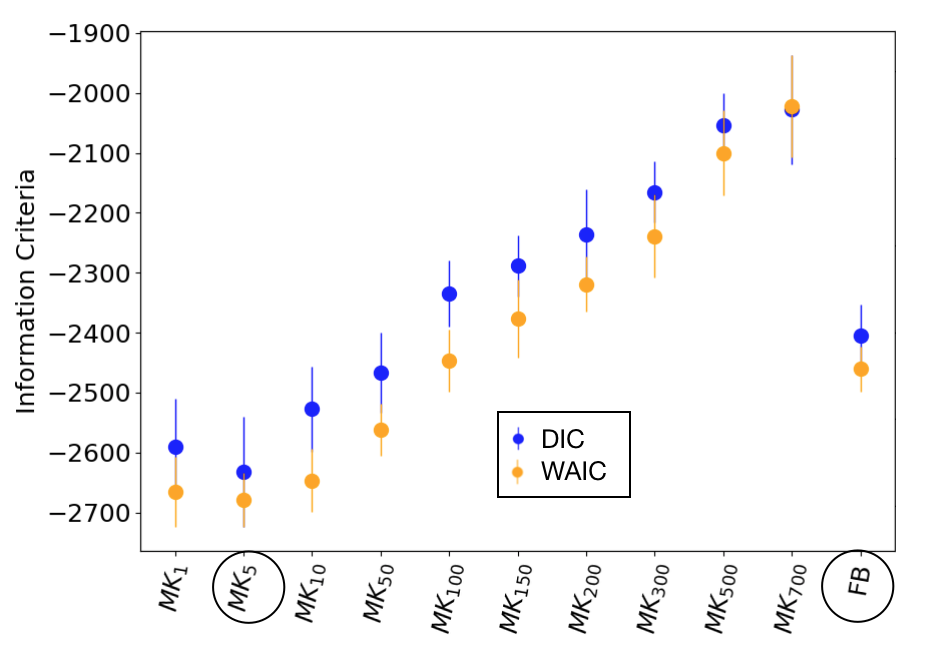
\includegraphics[width=0.48\textwidth]{images/dic_waic_scores.png}
\caption{DIC and WAIC as a function of the model (lower on y-axis is better). The $MK_5$ model is optimal, the $FB$ approach is in 5th place.}
%The DIC is the left y-axis and the WAIC is the right y-axis but it is the relative scores within each of these metrics that allows us to perform model comparison.}
\label{fig:dic_waic_scores}
\end{figure}

% The students may also release water from the Reservoir to direct to the Desert. 
%We use a model that segments time into these coherent periods where the parameters of the model describe the changing water levels. The output of the model is a number of periods that together span the entire session with CW and also describe the dynamics that occurred in CW.
% in time aids in describing the actions of students on the floor of CW. A major obstacle that was encountered in this previous work was one that is commonly encountered in clustering and unsupervised machine learning: How, a priori, to choose the number of clusters, or periods, to search for in the data.
% The students' activity (moving the physical logs to redirect water) directly influences the water levels in the simulation and we use the data log\footnote{Note the overloaded use of ``log''. ``Log'' can refer to the objects that the students move as well as the actual data logs. When context does not disambiguate these two cases, I will explicitly state whether I am referring to either ``physical'' or ``data'' logs.} files that record these water levels in the various areas of the simulation to represent the effects of the students' actions on the simulation outcomes. The logs are therefore a time series that 
%We solve this problem by employing Bayesian non-parametric methods where the cardinality of the latent space is learnt in tandem with the other model parameters. In particular, we use the sticky hierarchical Dirichlet process hidden Markov model (sticky HMM)~\cite{fox2008hdp,teh2005sharing} to learn latent stable states that the CW system adopts.
% \subsection{The sticky HMM}
% \label{sec:stickyhdphmm}

% This ``sticky'' parameter controls the expected number of inferred periods as it controls the degree to which the algorithm is biased to persist in a period (or state), given that it has already adopted that period/state. We are still required to choose this parameter and so two options are: (1) optimise statistical information criteria to evaluate the model on predictive tasks or; (2) place a weak prior on the parameter and perform a full Bayesian analysis (recommended by ~\cite{fox2009bayesian}). The work that follows shows that, for models that aim to assist human interpretation of the domain, the choice of hyperparameters in a model cannot merely rely on statistical measures of predictive performance.

% number of discrete latent states and transitions through these states as time progresses, is the hidden Markov model (HMM). Here a latent state directly corresponds to a period, the transitions between states correspond to the system changing between periods and the HMM emission distribution is a multivariate Gaussian that describes the first order difference in the  water levels in the different biomes of the simulation. Two problems with a vanilla HMM representation remain: (1) how to choose the cardinality of the state space; and (2) the HMM can allow rapid switching between states and therefore does not capture the notion of state persistence~\cite{fox2008hdp,fox2009bayesian,gruber2007hidden}.

%To address these two problems, we follow \citename{fox2008hdp}'s specification and employ the sticky HMM with multivariate Gaussian emission distributions to model the change in water levels in the four biomes of the Connected Worlds simulation.The alternative of \citename{hoernle2018modeling} introduced structure to the model to solve problem (2) but it could not address problem (1).

%\citename{fox2008hdp}'s architecture 

% \section{Method}
% % in this section we show how to take a model and data and find the interpretability.
% Previous work~\cite{chang2009reading,doshi2017roadmap} asserts that measurements for interpretability can be operationalised as a ``Forward Simulation'' task where people see a representation of a machine learning (ML) model's input and are asked to predict the label that the ML model would choose. If people can easily predict the model's output, on that specific instance, then the model is deemed interpretable for that instance. Another related interpretability test is the ``Binary Forced Choice''~\cite{doshi2017roadmap} where human test subjects are asked to select between two competing explanations for the observed test case. Again, if the people select the explanation that is generated by the model (as opposed to some decoy,) then the model is deemed interpretable on that data instance. We use these two operational definitions to test two hypotheses about the interpretability of a model which requires hyperparameter selection.

% First, in order to optimise an interpretabilty measure, we require that there exists some function that maps the parameter choice to an interpretability score. This function should be (locally) convex for there to exist a region in parameter space that corresponds to a high interpretability score. We test for the existence of this function. Second, we investigate how statistical approximations to this function should be used with caution when attempting to find the true optimal setting for human interpretability. We thus arrive at the following two hypotheses:

% \noindent \textbf{Hypothesis 1:} \textit{The degree to which a model is interpretable depends on the parameter settings; there exists a region in parameter space that corresponds to a high interpretability score.}

% \noindent \textbf{Hypothesis 2:} \textit{Optimising parameters for statistical information criteria may not produce the optimal model for human interpretability.}


\section{User Study} 
\label{sec:interpretability_results}

% \subsection{Selecting Periods from the Different Segmentations of the Data}
% \label{sec:select_segmentation}

% Each model ($M$) induces a unique segmentation of the data into a set of periods. Each period is a duration of time where the dynamics of the CW system are approximately stable according to $M$.

In this section we describe a user study that compares the interpretability of different models for describing the responses of the simulation to students' interactions in CW. 
The set of models includes the 12 CW models described in Section~\ref{sec:model_for_segmenting_time}.%; a time series $D$ consists of an 8-minute interaction sequence of students' activities.

%   first select 12 random points in time that remain constant across all model conditions. This results in approximately $1$ time point for every $40$ seconds of interaction. These $12$ points in time are used to select $12$ \textbf{candidate periods}. For a time point at $t$ seconds, a candidate period is chosen by finding the period from model $M$ that is active at time $t$. For example, if one of the $12$ points in time is $1min 42sec$ and we are generating the candidate period for $MK_1$, then we find the period from $MK_1$ that is active at the time $1min 42sec$. 

% Once the period segmentations per model have been generated, the times for selecting the candidate periods have been chosen and the candidate periods have been selected, we can move on to selecting the \textbf{intrusion periods}.

% An intrusion period is selected by choosing the neighbouring period to a candidate period. For each of the $12$ candidate periods that were selected, we select one intrusion period forward in time and one intrusion period backward in time. This ensures the test captures both sides of the candidate period in the event that one change of period is more ambiguous than another. Figure~\ref{fig:selection_representation}b also depicts the selection of a ``forward'' intruder. The set of all $(candidate, intruder)$ period selections gives $24$ experimental test cases per model for the given data set. This procedure for generating the experiment test cases is summarised the following pseudo-code. 
%The selection process is seen in detail in Figure~\ref{fig:selection_representation}b.

% \begin{figure}
% \begin{scriptsize}\begin{verbatim}

% Function SelectCandidate(model, data, time)
%     periods = model.getSegmentation(data)
%     activePeriod = periods[time]
%     Return activePeriod
% EndFunction

% Function SelectIntrusion(model, data, candidate, forward)
%     periods = model.getSegmentation(data)
%     If (forward)
%         period = <get forward neighbor to candidate>
%     Else
%         period = <get backward neighbor to candidate>
%     EndIf
%     Return period
% EndFunction

% experimentSamples = []
% selectedTimes = <randomly choose 12 time points>
% For M in Models:
%     For t in selectedTimes:
%         candidate = SelectCandidate(M, Data, t)
%         intrusioForward = SelectIntrusion(M, 
%                   Data, candidate, forward=True)
%         intrusioBackward = SelectIntrusion(M, 
%                   Data, candidate, forward=False)
%         experimentSamples.append((candidate, 
%                   intrusioForward))
%         experimentSamples.append((candidate, 
%                   intrusioBackward))
%     EndFor
% EndFor

% \end{verbatim}\end{scriptsize}
% \caption{Psudeocode for period selection}
% \end{figure}

% There are a total of $12 \times 24 = 288$ experiment test samples that need human labeling that together are used to infer an interpretability score ($IS$) per model on this data.
% TODO: ``This suggests that as topics become more fine-grained in models with larger number of topics, they are less useful for humans''
% 25 students total, 172 Mturkers
We recruited participants from two cohorts: undergraduate engineering students in a large public university
and Mturk workers (with a total of $240$ people who participated in the experimentation).
For a given data instance, we randomly sampled a set of 12 time points, which  remained constant across all model conditions.    
Each time point generated 2 experiment trials for each model, making $2 \times 12 \times 12=288$ trials per data instance. The reason for $2$ trials per time point is to select both the forward and backward intruders (in time) for each selected candidate period. Each participant saw 20 randomly sampled experiment trials, with no more than 2 trials from any given model, to ensure a representative range of models.  
After making their choice, participants received brief visual feedback on whether or not their selection was correct. 

All participants received a detailed tutorial about CW and the study, as well as a pre-study comprehension quiz\footnote{Tutorial pdf slides are available in the supplementary material.}. Mturk workers were paid a base rate of $\$0.25$ for participating and a bonus structure of $\$0.1$ for each correct response.


% \begin{table}[t]
%     \centering
%     \begin{tabular}{|c|c||c|c|}
%     \hline
%       Model  & FS (\% Acc.) & Model  & BC(\% Acc.) \\
%         \hline
%         $MK_{10}$ & 74.6    & $MK_{150}$  & 82.1  \\
%         $MK_{100}$ & 69.7   & $MK_1$      & 79.4  \\
%         $MK_{150}$ & 69.0   & $FB$        & 76.7  \\
%         $MK_{50}$ & 68.8    & $MK_{200}$  & 76.3  \\
%         \hline
%         \end{tabular}
%     \caption{Accuracy of most  interpretable models   \nh{TODO: Barbara found this table unintelligible - we need to be clearer about what we are saying}}
%     \label{tab:accuracy}
% \end{table}

% \begin{table}[t]
%     \centering
%     \begin{tabular}{|c|c||c|c|}
%     \hline
%       Test & Log File & Model & Accuracy (\%) \\
%         \hline
%         BFC       & 1       & $MK_{150}$      & $80.2$ \\
%         BFC       & 2       & $MK_{100}$      & $82.4$ \\
%         FS         & 1       & $MK_{10}$       & $73.7$ \\
%         FS         & 2       & $MK_{200}$      & $82.5$ \\
%         \hline
%         \end{tabular}
%     \caption{Top performing models (percent of instances labelled correctly) on each data instance for both Binary Forced Choice (BFC) and Forward Simulation (FS) tests.}
%     \label{tab:accuracy}
% \end{table}

% BFC: Best MK_{100} on dataset 2 with 82.4, and MK_150 on dataset 1 with  80.2
% FS: Best MK_{200} on dataset 2 with 82.5, and MK_10 on dataset 1 with  74.7


\begin{figure}[t]
% \centering
% 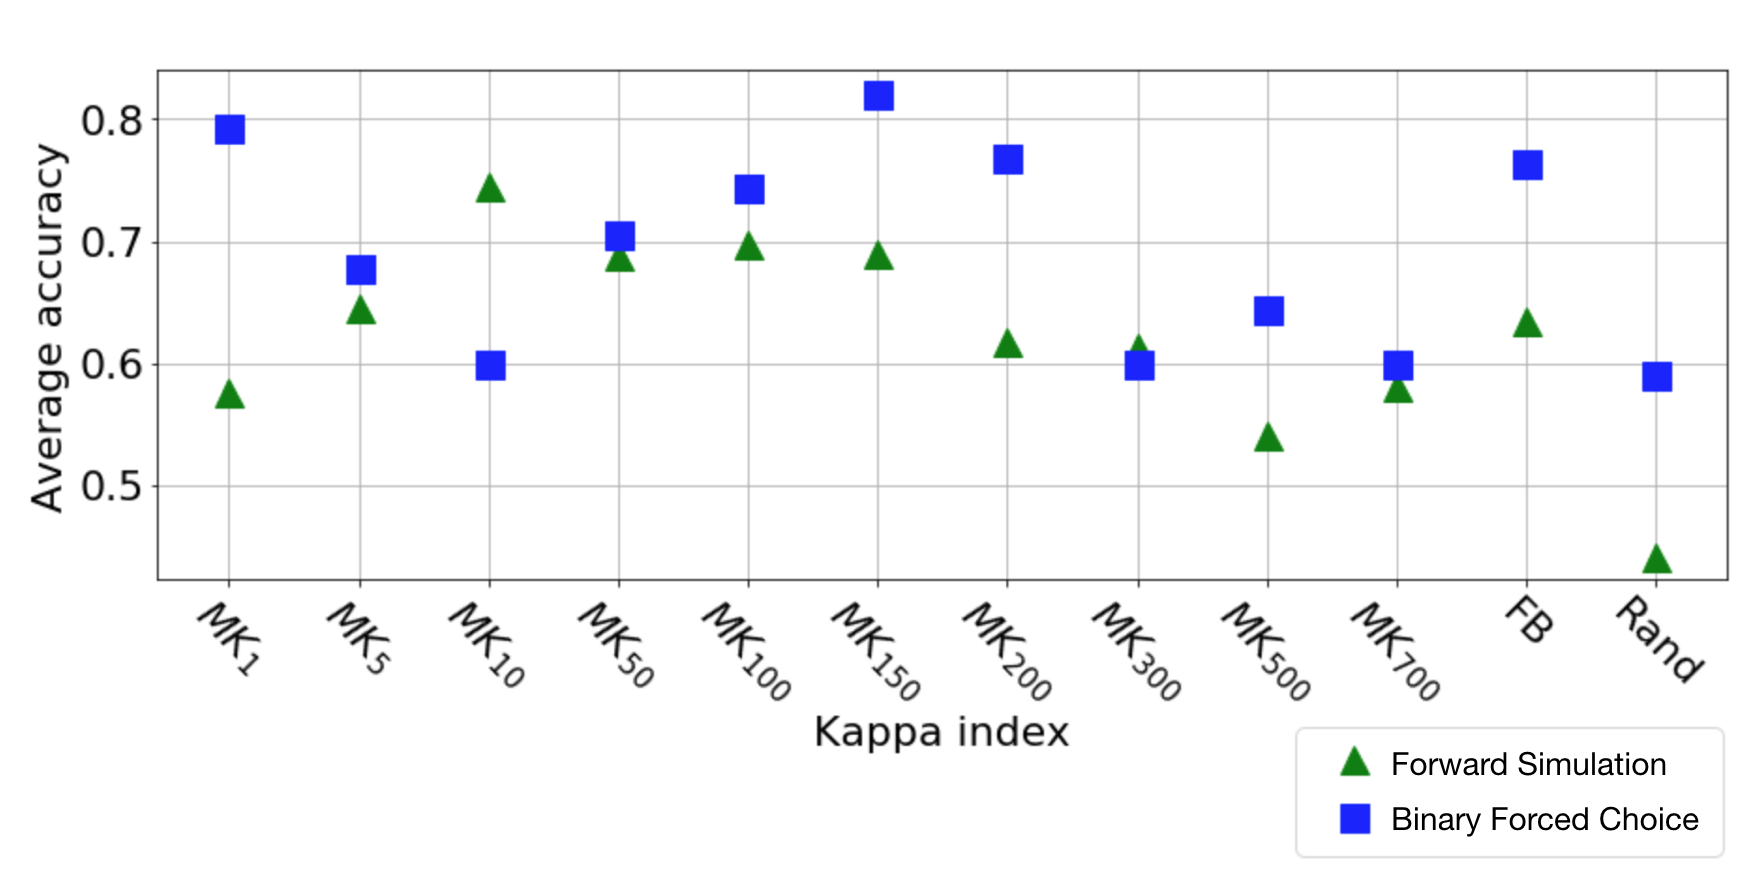
\includegraphics[width=.45\textwidth]{images/essil_combined_results_raw.png}
% \caption{Average accuracy for each model.}
% \label{fig:essil_test_results_raw}

% \vspace*{\floatsep}

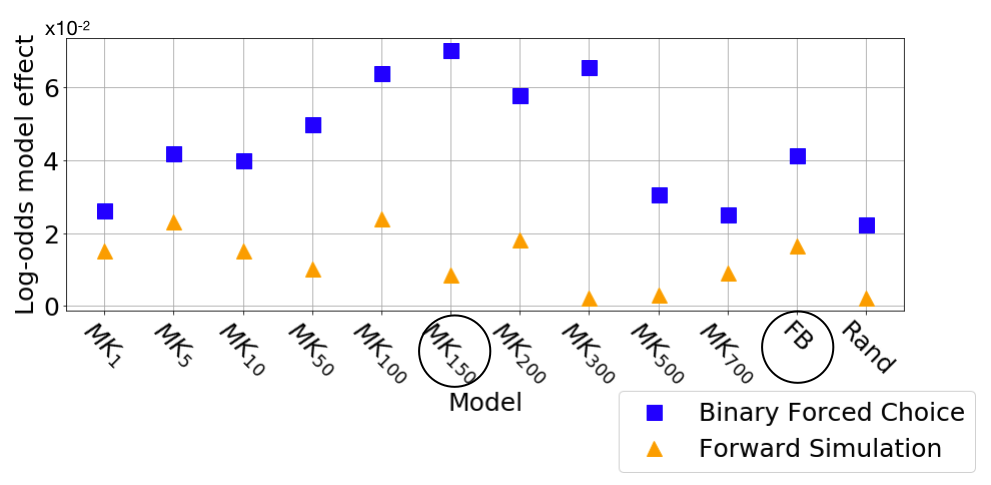
\includegraphics[width=.48\textwidth]{aaai_docs/images/combined_res_data_all.png}
\caption{Effect of each model on the log-odds of a test evaluator selecting the correct response (controlling for the test evaluator, the experiment trial, log file and ordering effects).}
\label{fig:essil_test_results}
\end{figure}

% TODO (Nick).
% Remove Table 1
% Put in new Figure 8
% Say in text
% Most accurate models from FS, BFC.
% Results from first instance exhibited a similar trend.

% The top models, in terms of raw accuracy are shown in :% $MK_{100}$ on dataset 2 with 82.4, and MK_150 on dataset 1 with  80.2
% FS: Best MK_{200} on dataset 2 with 82.5, and MK_10 on dataset 1 with  74.7
We first describe results in terms of accuracy (the percent of correctly labelled test instances). 
The top performing model was $MK_{200}$ with an accuracy of $83\%$ on the Forward Simulation  test and $MK_{100}$  with an accuracy of $82\%$ on the Binary Forced Choice test. 
The random baseline model performed consistently poorly with an average accuracy of $53\%$ on both tests. 
The fully Bayesian model achieved an accuracy of $72\%$ and $70\%$ respectively on the two tests. 
% each model by averaging  the number of correct test responses over all  experiment trials 
% for that model.  

To control for ordering effects, chosen time periods, data instance used, and effects of individual participants, we applied an L2 regularized logistic regression for predicting  the user specific success on the experiment trial, shown  in  Figure~\ref{fig:essil_test_results}. The y-axis presents the improvement in log-odds that a model has on the expected response accuracy (higher is better). 
As shown by the figure,  the Forward Simulation shows a high variance with no clear maximum. In contrast, the Binary Forced Choice test has a clear maximum in the region of $MK_{100}$ and $MK_{150}$.
%These models also  maximized the raw accuracy. 
%All of the models ($MK_{1},\ldots,MK_{700}, FB$) show an improvement over the random model (with a score of close to $0$). 
%Notice too that the fully Bayesian model appears to perform well on both tests (being in the top $4$ models in the Forward Simulation and in the top $6$ models for Binary Forced Choice).
%Greater values on the y-axis mean there is a higher likelihood that the model is interpretable. 

From both Figures~\ref{fig:dic_waic_scores} and~\ref{fig:essil_test_results} we can infer the following four conclusions. 
First, all of the models ($MK_{1},\ldots,MK_{700}, FB$) outperform the random baseline: participants are more likely to select the correct response from any of these models. This result suggests that periods of stable dynamics  exist in the data and that it is possible to construct models, which describe these dynamics, that are interpretable to people. 

Second, the Binary Forced Choice test is a preferable measure for interpretablity   to the Forward Simulation test. Figure~\ref{fig:essil_test_results} shows that the Binary Forced Choice test exhibits a clear peak (around $MK_{100}$ and $MK_{150}$) where interpretability of the model is maximized. 
These models also maximized the  raw accuracy on the Binary Forced Choice test.

On the other hand, the Forward Simulation test has a greater variance across models and across data instances. 
Two possible causes for this higher variance are: (1) there is more room for error in the Forward Simulation test (5 choices vs. 2 choices in Binary Forced Choice); (2) sampling a single image to represent a period (as in Forward Simulation) presents less information to the user than sampling 4 images (as in Binary Forced Choice). 
%the 4 images provide a better representation of a period because they are less  prone to the noise that using only one image to represent a period might engender. %However, the 4 image representation is less prone to sampling 1 poor image (as is the case in the Forward Simulation) thereby making this the preferable test.
% Table~\ref{tab:accuracy} shows that scores were generally higher on the Binary Forced Choice test than on the Forward Simulation. This is natural because (1) there are only two choices in the Binary Forced Choice as opposed to five in the Forward Simulation and (2) both the intrusion and the candidate periods are represented by $4$ images each, making the visualisations less prone to the noise that using only one image to represent a period might engender. However, the 4 image representation is less prone to sampling 1 poor image (as is the case in the Forward Simulation) thereby making this the preferable test.
% The most interpretable models from Figure~\ref{fig:essil_test_results} ($MK_{100}, MK_{150}$) obtain an accuracy above 80\% on the Binary Forced Choice test. The variance of the results from the Forward Simulation test is high. For example, $MK_{150}$ achieves a raw accuracy of $69\%$ on data instance 1, on data instance 2 the accuracy is only $60.3\%$.

Third, the best $\kappa$ settings vary for different tests and information criteria. 
Model interpretability grows steadily as the value of $\kappa$ increases, with $MK_{100}$ and $MK_{150}$ being the optimal models, and then proceeds to decrease steadily.   
These models are not consistent with the model $MK_5$ that optimized the information criteria.
Note that higher $\kappa$ values are ``sticky'' - they  bias the model towards longer periods, which condense too many activities to make sense to people. 
On the other end of the spectrum, lower $\kappa$ values allow for shorter periods that capture too much of the noise in the system.  
In contrast, the $\kappa$ value for  models $MK_{100}$ and $MK_{150}$ 
represent a ``sweet spot" in between these two extremes.
%Both ends of the $\kappa$ scale represent less interpretable models than the ``sweet spot" that is represen.

% In contrast, lower values 
% are   optimal when considering statistical information criteria. 
% Specifically, $MK_{100}, MK_{150}, MK_{50}$ are all within the top 4 models when optimzing for interpretability score (accuracy and log-odds ratios), while 
% $MK_5, MK_1$ and $MK_{10}$ are within the top 4 models when optimizing information score (DIC and WAIC).  
 
Finally, the fully Bayesian model $(FB)$ performs consistently well on both information criteria and interpretability tests. It is interesting to note that while this model does not find the optimal setting (from neither the statistical information criteria nor from the human interpretability task) it does perform well across all tests, tasks and instances, and is fully automated (no human evaluation is required in order to choose an optimal parameter setting).

We conclude this section with mentioning the limitation that the user study was based on a small number $(n=2)$  of instances. This was due to the difficulty in obtaining controlled sessions of student behavior in CW. Despite this issue, the differences between the models in Figure~\ref{fig:essil_test_results} are statistically significant, having being evaluated across 12 different time points for each instance and with hundreds of evaluators.
% Investigating the application of this result could form the basis for interesting future work (i.e., it is possible that the most robust solution is to use the fully Bayesian model in all cases. The implications for \cite{chang2009reading} would be to implement a hierarchical Dirichlet process model to compare to the LDA that was presented).
 
%  Lastly, the Binary Forced Choice test is a preferable measure for interpretablity in our domain to the Forward Simulation test. Table~\ref{tab:accuracy} shows that scores were generally higher on the Binary Forced Choice test than on the Forward Simulation. This is natural because (1) there are only two choices in the Binary Forced Choice as opposed to five in the Forward Simulation and (2) both the intrusion and the candidate periods are represented by $4$ images each, making the visualisations less prone to the noise that using only one image to represent a period might engender. However, the 4 image representation is less prone to sampling 1 poor image (as is the case in the Forward Simulation) thereby making this the preferable test.
 %In Table~\ref{tab:accuracy}, the $MK_1$ model performs well on the Binary Forced Choice test and very poorly on the Forward Simulation test. Using evidence from Figure~\ref{fig:essil_test_results}, we conclude this was because $MK_1$ in the Binary Forced Choice condition happened to get test subjects who were good at labelling the correct explanation. When we control for the ``skill'' of the test subject, we see this difference is substantially smaller. 
 
%  Controlling for the variable factors listed above helps to show in Figure~\ref{fig:essil_test_results} that the optimal setting for $\kappa$ exists between $50$ and $150$.
 %We also clearly see how the random model performs poorly. 
%  Lastly, a notable results is that the fully Bayesian model performs well on both experiments. 

% The following analyzes results from 145 participants (128 Mturkers and 17 students) who achieved more than 50\% correct responses, and spent between 2 and 10 minutes on the task.  

% experiments on Amazon Mechanical Turk (Mturk) where we recruited $87$ and $85$ Mturk workers (turkers) for the Forward Simulation and the Binary Forced Choice experiment respectively. Each turker sees $20$ experiment trials where a progress bar is presented to track their progress through the $20$ trials. Of the $20$ trials, the turker sees a maximum of $2$ trials from any one setting of model and thus each turker sees a range of representations from a range of models. After selecting the choice for each intruding image, the turkers receive brief visual feedback on whether or not their selection was correct. 

% Results were discarded from both experimental conditions if (1) the turkers were correct on fewer than $12$ responses or (2) took less than 2 minutes to complete the task or more than 10 minutes. We remain with $66$ and $62$ turkers respectively. Before the turkers are given access to the experiment, they are shown a slide show which describes the CW system and how students work to control the system dynamics. They are also given a detailed tutorial about the user interface and they are required to pass a comprehension quiz which tests whether they read and understood the slideshow. If a turker fails the quiz, he is blocked from participating in the experiment.

% A brief validation of the time-on-task, shown in Figure~\ref{fig:time_to_complete_task}, shows that turkers decreased the amount of time required to answer an experiment trial as they progressed through their tasks from 1 to 20. It is natural that the first tasks took the turkers longer as they were still becoming comfortable with the domain.

% \begin{figure}[t]
% \centering

% \end{figure}


% \begin{figure}[h]
% \centering
% 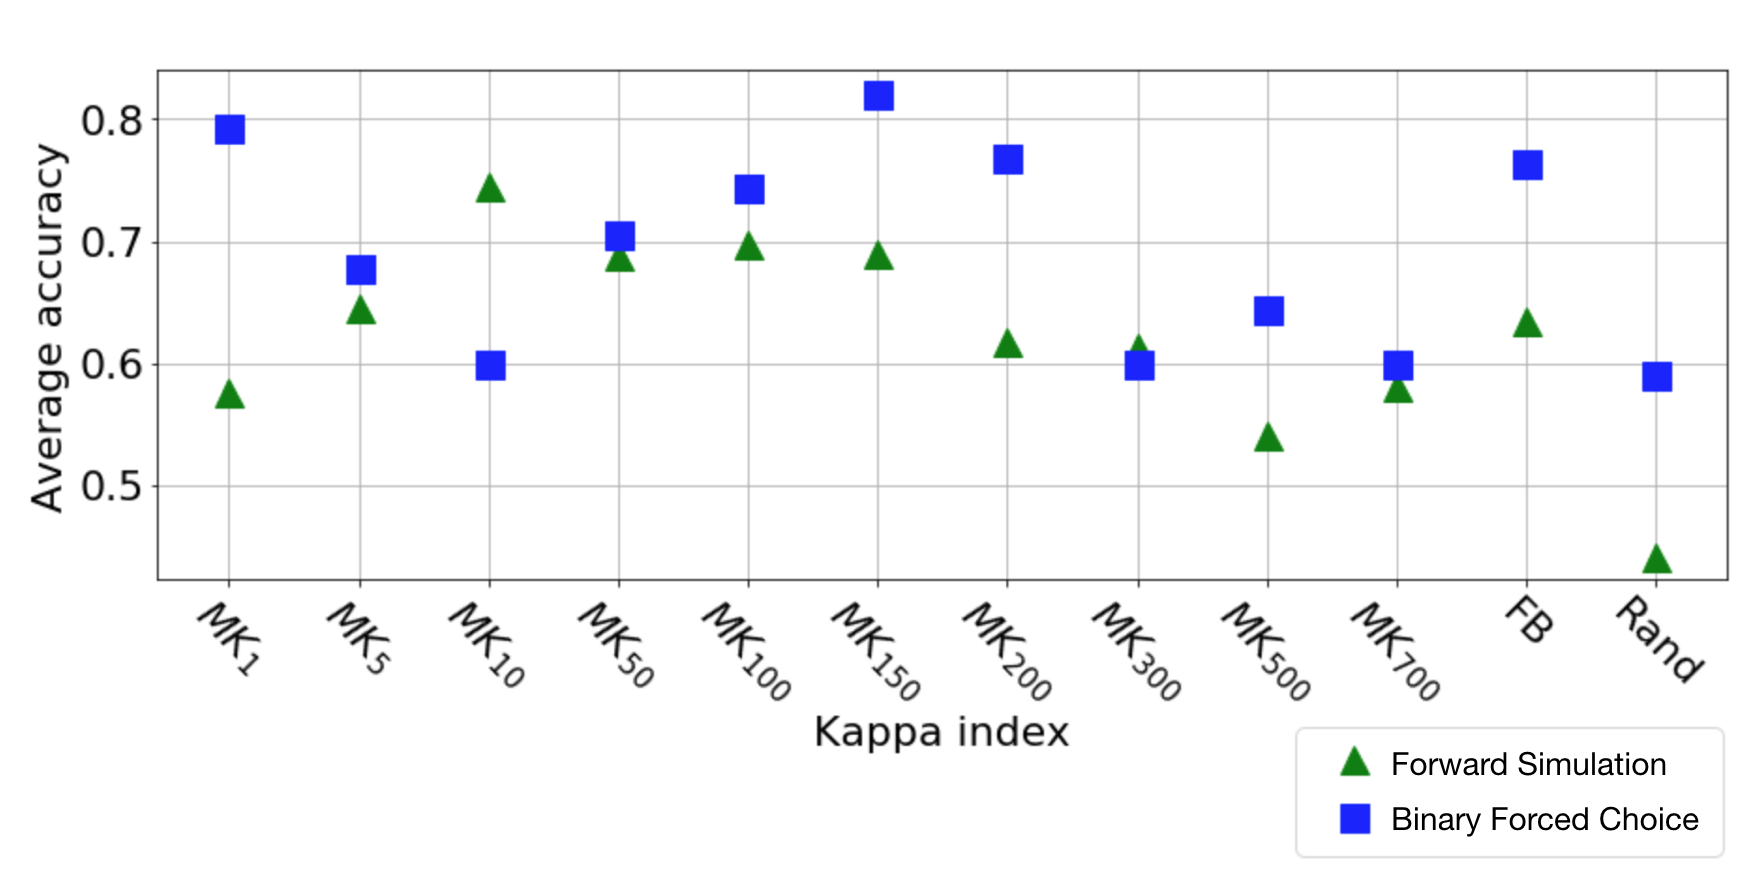
\includegraphics[width=\textwidth]{images/essil_combined_results_raw.png}
% \caption{}
% \label{fig:essil_test_results_raw}
% \end{figure}

% \includegraphics[width=.75\textwidth]{images/time_to_complete_task.png}
% \caption{Time to complete an individual task. Initially, the turkers take longer to complete the tasks as they are still unfamiliar with the domain. The time to complete a task tends toward approximately 10 seconds per task for both tests.}
% \label{fig:time_to_complete_task}

% \vspace*{\floatsep}


% Figures~\ref{fig:essil_test_results_raw} and \ref{fig:essil_test_results} present the main results from the experiment. Figure~\ref{fig:essil_test_results_raw} shows the average accuracy of each model without controlling for any variation between the experiments that a user sees and how accurate that user is. 


% In Figure~\ref{fig:essil_test_results}, 


% (1) the user who labelled an instance, (2) the experiment trial (i.e., where in time the candidate period was selected from and whether the intruder was forward or backward in time), (3) the order in which the user saw the instance, and (4) the model that was used to generate the trial. This was done by running a L2 regularised Logistic Regression to predict the user specific success on the experiment trial. The y-axis therefore presents the effect in change of log-odds that the model had on the expected success of selecting the correct response. Greater values on the y-axis mean there is a greater likelihood that any trial from the model's segmentation is correct. Both the raw accuracy (in Figure~\ref{fig:essil_test_results_raw}) and the log-odds effect of the model (in Figure~\ref{fig:essil_test_results}) are examples of an interpretability score ($IS$) in this domain. The $IS$ is a relative score and in each case, the models with the highest scores are deemed optimal.

% % The logistic regression model is shown in Equation~\ref{eq:logistic_regression_of_results} where $p_{j}$ refers to the probability of success on a particular trial $j$ where turker $t$ makes a decision on experiment trial $i$ from model $m$ and saw this trial in position $o$. There is a constant effect $\alpha$ that controls for the difficulty of the experiment (the intrusion test is harder than the binary controlled test), $\beta_u$ is the user specific ``skill'' parameter, $\beta_m$ is the effect that the model has on the probability of a correct response (and is the parameter of interest), $\beta_i$ controls for the difficulty of the experiment trial (i.e., did the points in time vary in their difficulty) and $\beta_o$ controls for the order in which that instance was seen. $\mathds{1}$ is an indicator function that evaluates to $1$ if the argument is true and $0$ otherwise.

% \begin{equation}
%     \label{eq:logistic_regression_of_results}
%     \log(\frac{p_{j}}{1-p_{j}}) = \alpha + \sum\limits_{t=1}^{T}\beta_u\mathds{1}(turker=t)+ \sum\limits_{m=1}^{12}\beta_m\mathds{1}(model=m)+ \sum\limits_{i=1}^{24}\beta_i\mathds{1}(trial=i)+ \sum\limits_{o=1}^{20}\beta_o\mathds{1}(order=o)
% \end{equation}

%TODO: need to use IS here


% There are three main conclusions that can be drawn from the results, two of which support previous work and one of which is novel. All of the parameters in the regression were significant (however, due to the large sample size this is unsurprising).
% \begin{enumerate}
%     \item All of the parameterised models outperform the random baseline: turkers are more likely to select the correct response from any of these models. This result suggests that periods of stable dynamics do indeed exist in the data and using an algorithm that finds the periods and the boundaries between the periods is useful for representing the dynamics of the system. This result confirms the previous results of \cite{hoernle2018modeling}.
%     \item The optimal model for interpretability appears to be in the region of $MK_{10}$, $MK_{50}$, $MK_{100}$ or $MK_{150}$. All of these models under-perform the optimal model $MK_{5}$ on the DIC and WAIC information criteria metrics and therefore would not be selected if our only metric was to optimise these statistical tests. This result confirms previous work~\cite{chang2009reading, doshi2017roadmap} however, it does contribute to the evidence of this problem by studying this unique time series domain.
%     \item The fully Bayesian model performs consistently well on both statistical tests and on both of the interpretability tests. It is interesting to note that while this model does not find the optimal setting (from neither the statistical information criteria nor from the human interpretability task) it does perform consistently well across both tasks. Investigating the application of this result could form the basis for interesting future work (i.e., it is possible that the most robust solution is to use the fully Bayesian model in all cases. The implications for \cite{chang2009reading} would be to implement a hierarchical Dirichlet process model to compare to the LDA that was presented).
% \end{enumerate}

% \noindent We therefore accept both hypotheses. First, from Figure~\ref{fig:essil_test_results}, it is apparent that there does exist some area of the setting of the parameter $\kappa$ that does correspond to a consistently high interpretability score. Second, in Figure~\ref{fig:dic_waic_scores}, we see that the statistical theory would choose model $MK_5$ as the optimal model. This clearly does not correspond to the optimal model in neither Figure~\ref{fig:essil_test_results_raw} nor in Figure~\ref{fig:essil_test_results}.

\section{Conclusion \& Future Work}
% \nh{this is probably too far afield - especially for socially relevant track... anyway, it is an idea for work...}
% The Bayesian non-parametric technique used to perform inference over the latent cardinality of the state-space has applications in many areas. Most notably,~\cite{teh2005sharing} showed that this model achieves better log-likelihood on text data, than its parametric cousin: Latent Dirichlet Allocation~\cite{blei2003latent}. \cite{chang2009reading} showed that the cardinality of the LDA model with optimal log-likelihood did not correspond to the model that was deemed most interpretable by people. From the results in this paper, we suggest an experiment that compares the Bayesian non-parametric (hierarchical Dirichlet process) to LDA with a varying state-space.

% We are akready using visualisation for use in the classroom, where teachers ... to reflect on their interactions... to raise discussions...

With the growing prevalence of immersive simulations so arises the need for AI systems which help end-users gain insight into the activities of the participants. 
We have studied an environmental simulation where students learn about the causal effects of their actions. 
Our results show that algorithms can segment time series log data into periods that are coherent for people. 
However, selecting hyperparameters in these models is a challenge, especially when trying to optimize the representations for their interpretability.
We have shown an example of how to select these hyperparameters from two tests that are grounded in the literature and we have further presented the fully Bayesian method as promising technique for implementing a model when human evaluations are not possible. 
Future work will apply these models to alternative domains and will work with teachers and experts ``in the loop'' such that we can target the goal of engaging the participants with insights drawn from their own experiences with such immersive simulations.
% Future work will apply similar models to alternative domains and will include system experts such that we can complete the loop on using the inference algorithms to present useful feedback to these participants. 
% From Leilah: such that we can engage participants with while they are still immersed in the simulation, allowing model results to formatively guide their continued interactions.

\bibliographystyle{aaai.bst}
\bibliography{bibliography}
\end{document}

% TODO: 
% - Defend held-out log-likelihood
% - levers: which images, which periods
% - non-supervised learning

% TODO (nick): paragraph about kappa sticky parameter (higher biases more persistence)
% TODO (nick): selection of periods intruder and candidate is conservative (we select periods that are right next to one another)
% TODO (nick): explain Bayesian vs Full Bayesian
% TODO: look at the BGU class feedback
% TODO: do the turkers improve over time
% TODO: expand the experiment to include another trial
% TODO: table model name, fwd sim acc, bfc acc
% TODO: FWD sim gives more variance on the selection of any one image. BFC gives equal weight to the representations of the two experiments.
% TODO: results are statistically significant
% TODO: comments from students and workers.

% COMMENTS:
% ---------------------------------------
% I evaluated all three water sources and tried from there.
% Worked well. I'm not sure how to answer "how" I got my answers. I constructed a narrative for both possibilities and looked for how the target image might fit into either "story."
% I tried to find one image in all the images that was the closest to the one in the center and selected that period
%  Mostly I tried to identify the position of the  logs, then tried to match the water flow pattern. Thank you and good luck with your results.
% I first kept trying to see which biomes were receiving water and which weren't and based answers off that and had little success and eventually just started paying no attention to the biomes and instead just taking a broad look at all the images and trying to find which ones sort of looked alike, and began having success. 
% I based a lot of my decisions off of the placement of the red logs. Then I tried to imagine how the water would flow. Last I selected the group that seemed to fit most with #1 log placement, then #2 water flow.
% It was comparison on a multipoint basis. I picked the one that had most biome comparisons. I still messed up a few times, but was slowly getting faster and better as I progressed.
% It was interesting but I think better results would be achieved if  It has 10  items istead 20
% I did better when i sat back a bit and got a view of all of them rather than looking at the details of which zones got water I think. Either way I think I'm dumb now haha...ha..
% some instances were easier but for some periods 1 and 2 were fairly similar so it was quite hard to tell which one it should be

% Figure~\ref{fig:essil_test_results} presents the main results from the experiment. To control for (1) the user who labelled an instance, (2) the experiment trial (i.e., where in time the candidate period was selected from and whether the intruder was forward or backward in time), (3) the order in which the user saw the instance, and (4) the model that was used to generate the trial, we ran a L2 regularised Logistic Regression to predict the user specific success on the experiment trial. The y-axis therefore presents the effect in change of log-odds that the model had on the expected success of selecting the correct response. Higher means there is a greater likelihood that a specific trial generated from that model's segmentation is correct.

% The logistic regression model is shown in equation~\ref{eq:logistic_regression_of_results} where $p_{j}$ refers to the probability of success on a particular trial $j$ where turker $t$ makes a decision on experiment trial $i$ from model $m$ and saw this trial in position $o$. There is a constant effect $\alpha$ that controls for the difficulty of the experiment (the intrusion test is harder than the binary controlled test), $\beta_u$ is the user specific ``skill'' parameter, $\beta_m$ is the effect that the model has on the probability of a correct response (and is the parameter of interest), $\beta_i$ controls for the difficulty of the experiment trial (i.e., did the points in time vary in their difficulty) and $\beta_o$ controls for the order in which that instance was seen. $\mathds{1}$ is an indicator function that evaluates to $1$ if the argument is true and $0$ otherwise.

% \begin{equation}
%     \label{eq:logistic_regression_of_results}
%     \log(\frac{p_{j}}{1-p_{j}}) = \alpha + \sum\limits_{t=1}^{T}\beta_u\mathds{1}(turker=t)+ \sum\limits_{m=1}^{12}\beta_m\mathds{1}(model=m)+ \sum\limits_{i=1}^{24}\beta_i\mathds{1}(trial=i)+ \sum\limits_{o=1}^{20}\beta_o\mathds{1}(order=o)
% \end{equation}